\chapter{BDT based $D^0$ analyses for the EIC}
\label{ch.results}

This chapter presents the methods and results of the machine learning analyses we performed to separate $D^0$ signals from background. In Ch. \ref{sec.results_gen_methods}, we outline the general analysis methodology and workflow common to all our analyses. In Ch. \ref{sec.results_bkg_study}, we present a preliminary analysis on the impacts of machine-background on $D^0$ invariant mass reconstruction, which we perform by applying an existing BDT framework to new data samples. Then in Ch. \ref{sec.results_optimization}, we present the steps taken to further optimize the framework for our analysis, in terms of the various aspects of BDT implementation discussed in Ch. \ref{sec.ml_implementation}, and discuss our findings.

%---------------------------------------------------------
\section{General methodology}
\label{sec.results_gen_methods}

All data is obtained from PYTHIA-8 simulated $ep$-collisions with $Q^2>1~{\rm GeV^2}$, which are provided by the ePIC Collaboration (ref. in Appendix \ref{app.samples}). We adapt the codes for obtaining $D^0$ signal and background candidates from \cite{Shyam_analysis}, and the machine learning framework from \cite{Shyam_ml}, provided by Shyam Kumar.

We obtain true signal candidates from $D^0$-enriched data samples, in which every collision event produces at least one $D^0$-meson. This rate of $D^0$ production is far above that expected in real $ep$ collisions, but we use this data in order to obtain sufficient signal candidates for training the BDT. We obtain the true background from minimum-bias DIS data samples, meaning that there is no $D^0$-enrichment. We will refer to the $D^0$-enriched data as ``D0 samples" and the minimum-bias data as ``DIS samples."

We combine signal and background candidates into one dataset $\mathcal{D}$, in which each candidate is represented by a vector containing the values of their topological features. We include the same number of signal and background candidates in $\mathcal{D}$ to avoid introducing bias. From $\mathcal{D}$, we randomly select 80\% of the data for $\mathcal{D}_{\rm train}$ and 20\% of the data for $\mathcal{D}_{\rm test}$.

Since we do not have real data to analyze, we estimate the BDT performance by ``applying" the model back on the original data $\mathcal{D}$. For a chosen BDT threshold, we calculate the resulting signal and background {\it efficiencies}, $\epsilon_{\rm{sig}}(\hat{y}^*)$ and $\epsilon_{\rm{bkg}}(\hat{y}^*)$, which are the percentages of signal and background candidates in the test dataset which are accepted by the model for a given BDT threshold $\hat{y}^*$. More concretely, if we start with a dataset $\mathcal{D}$ with $N^{\rm tot}_{\rm sig}$ signal candidates and $N^{\rm tot}_{\rm bkg}$ background candidates, then when we apply the BDT, we select the subset $\mathcal{D}^{\rm ML}$ that contains 
\begin{equation}
\begin{aligned}
    N^{\rm ML}_{\rm sig} &=\epsilon_{\rm sig}(\hat{y}^*) N^{\rm tot}_{\rm sig} \ , \\
    N^{\rm ML}_{\rm bkg} &=\epsilon_{\rm bkg}(\hat{y}^*) N^{\rm tot}_{\rm bkg} \label{eqn.eff}
\end{aligned}
\end{equation}
signal and background candidates.

In order to examine the effectiveness of the signal-and-background separation, we plot the invariant mass distribution of the combined signal and background candidates and look for the $D^0$ peak, which is located around 1.84 ${\rm GeV/c^2}$. For more realistic results, we first use a random sampling method 
(described in Appendix \ref{app.data_prep}) 
to scale up the number of candidates such that they correspond to the expected number of events in EIC experiments, with the desired luminosity of $10~{\rm fb}^{-1}$. We then calculate the S/B (Eq. \eqref{eqn.s_over_b}) and Significance (Eqn. \eqref{eqn.signif}) of the candidates in the $D^0$ peak region, defined to be within two standard deviations on either side of the peak value. We first determine the invariant mass distribution, S/B, and Significance for the initial data before using BDT (using $N_{\rm sig}^{\rm tot}$ and $N_{\rm bkg}^{\rm tot}$), then examine the improvements to these results after applying the BDT (using $N_{\rm bkg}^{\rm ML}$ and $N_{\rm bkg}^{\rm ML}$ ).

%---------------------------------------------------------
\section{Machine-background effects on $D^0$ invariant mass reconstruction: a preliminary analysis}
\label{sec.results_bkg_study}

As a preliminary study, we apply the BDT framework developed in previous work \cite{Shyam_ml} to two new sets of simulated data samples, one set with machine-background effects and one set without those effects. The goal of this study is to examine the impacts of machine background on the $D^0$ analysis. These machine-background effects include interactions between beam particles and gas in beam pipe, electron scattering within the beam, and synchrotron radiation \cite{eic_ptdr}, which produce additional noise in detector measurements. We aim to explore how these effects impact the effectiveness with which BDTs can separate the $D^0$ signals from background by comparing results for data with machine-background effects to those for data without those effects.

%-------------------------
\subsection{Preliminary BDT framework}
\label{sec.results_prelim_methods}

In this preliminary study, we analyze one set of D0 and DIS samples from simulations incorporating machine-background effects, along with a second set of D0 and DIS samples from data without those effects (ref. in Appendix \ref{app.samples}).

We separately train two BDT models---one model for the samples without machine-background effects, and another for the samples with those effects. Here, we analyze all the data in one inclusive kinematic range of $-2<y<3$ and $p_T>1$. We utilize the following 10 topological features, which characterize the $D^0\rightarrow\pi+K$ decay, depicted in Fig. \ref{f.d0_decay_diagram_2}:
\begin{multicols}{2}
\begin{itemize}
    \item \texttt{costheta}: $\cos{\theta}$
    \item \texttt{costheta\_xy}: $\cos{\theta_{xy}}$
    \item \texttt{decay\_length}: Decay Length
    \item \texttt{dca\_D0}: $\rm DCA_{D0}$
    \item \texttt{d0\_pi}: $\rm DCA_\pi$
    \item \texttt{d0\_k}: $\rm DCA_K$
    \item \texttt{d0xy\_pi}: ${\rm DCA_\pi}_{(xy)}$
    \item \texttt{signif\_d0xy\_pi}: ${\rm DCA_\pi}_{(xy)}/\sigma_\pi$
    \item \texttt{signif\_d0xy\_k}: ${\rm DCA_K}_{(xy)}/\sigma_K$
    \item \texttt{sigma\_vtx}: $\sigma$ of decay vertex
\end{itemize}
\end{multicols}
where $\sigma$ represents the associated uncertainty for a given variable. Often, the variables normalized by $\sigma$ may be provide more accurate representations of signal vs. background candidates. The \texttt{sigma\_vtx} feature is the uncertainty associated with the decay vertex location, where the vertex is taken to be the midpoint of the line defining ${\rm DCA_{12}}$. 

%
\begin{figure}[h!]
    \centering
    \includegraphics[width=0.6\linewidth]{gallery/D0_topology/d0_decay.png}
    \caption{$D^0\rightarrow \pi^+ + K^-$ decay in the transverse plane. The labelled topological features are defined in Ch. \ref{sec:def_top_vars}. Figure from the STAR Collaboration \cite{STAR}.}
    \label{f.d0_decay_diagram_2}
\end{figure}
%

We do not include all the available topological features, but adopt the preferred combination of features as determined in previous work. When applying the BDT model, we choose a threshold BDT output of 0.6, which is also the best value determined in previous work.

Here, we note that the particular kinematic range, topological feature selection, and BDT threshold are choices that have been optimized for previous work analyzing different data, so these choices are likely not the most effective for our analysis. In the subsequent analyses of Ch. \ref{sec.results_optimization}, we aim to optimize these choices for our particular data samples.


% \begin{equation}
%     eff_{\rm sig(bkg)} = \frac{N_{\rm sig(bkg)}\left[\hat{y}>\hat{y}^* \right]}{N_{\rm sig(bkg)}\left[\hat{y}\geq 0 \right]} \ ,
% \end{equation}
% where the numerator is the number of candidates accepted by the BDT for a given threshold $\hat{y}^*$, and the denominator is the total number of candidates/ 

%-------------------------
\subsection{BDT training}

To assess the performances of the BDT models, we examine the BDT outputs and ROC curves for the training vs. testing datasets, which we introduced in Ch. \ref{sec.ml_performance}.

%
\begin{figure}[h!]
    \centering
    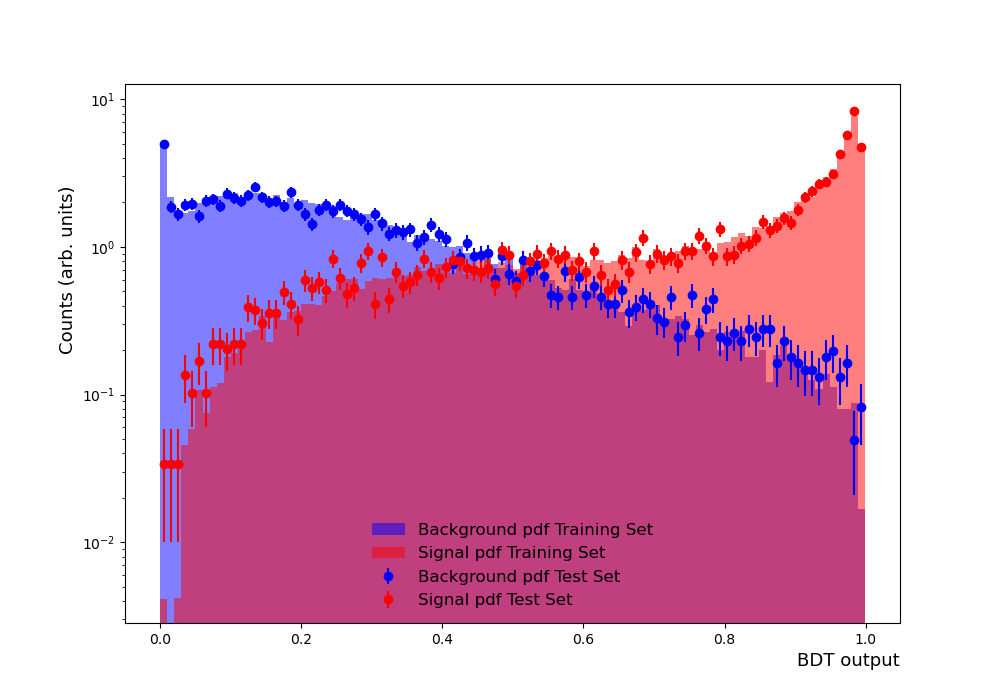
\includegraphics[width=0.5\linewidth]{gallery/results/train_test_without_bkg.png}
    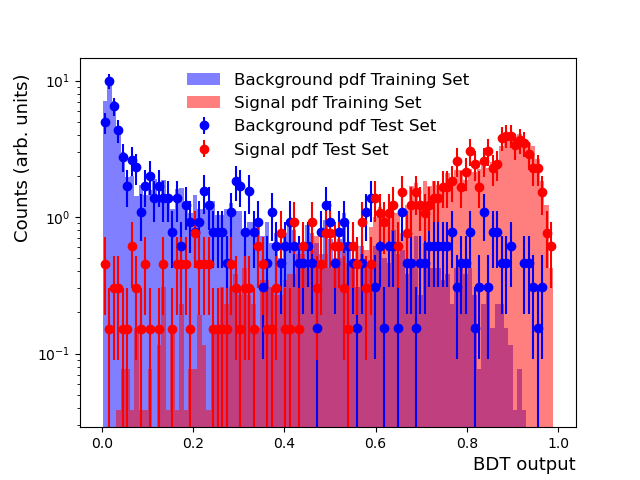
\includegraphics[width=0.46\linewidth]{gallery/results/train_test_with_bkg.png}
    \caption{BDT output distributions of training vs. test data for samples without (left) and \textbf{with (right)} machine-background effects. In both plots, training data are plotted as shaded histograms and test data are plotted as solid markers, with background candidates in blue and $D^0$ signal candidates in red.}
    \label{f.bkg_study_bdt_score}
\end{figure}
%
Fig. \ref{f.bkg_study_bdt_score} compares the BDT output distributions for the samples with and without machine-background effects. In the results for samples without machine-background effects (left plot), we observe that the distributions for training and testing data follow each other closely, which indicates that the BDT model results are consistent across both datasets. However, for the samples {\textbf{with}} machine-background effects (the right-side plots), we notice much greater discrepancy between the outputs for training and testing data near the tail ends of each distribution, which indicates that the model is less stable. We also see that the distributions for the samples {\textbf{with}} machine-background effects are less strongly peaked near 0 and 1, which suggests that the discriminatory ability of this BDT model is weaker. This is likely because the topological distributions of signal and background look more similar as a result of the machine-background effects.

%
\begin{figure}[h!]
    \centering
    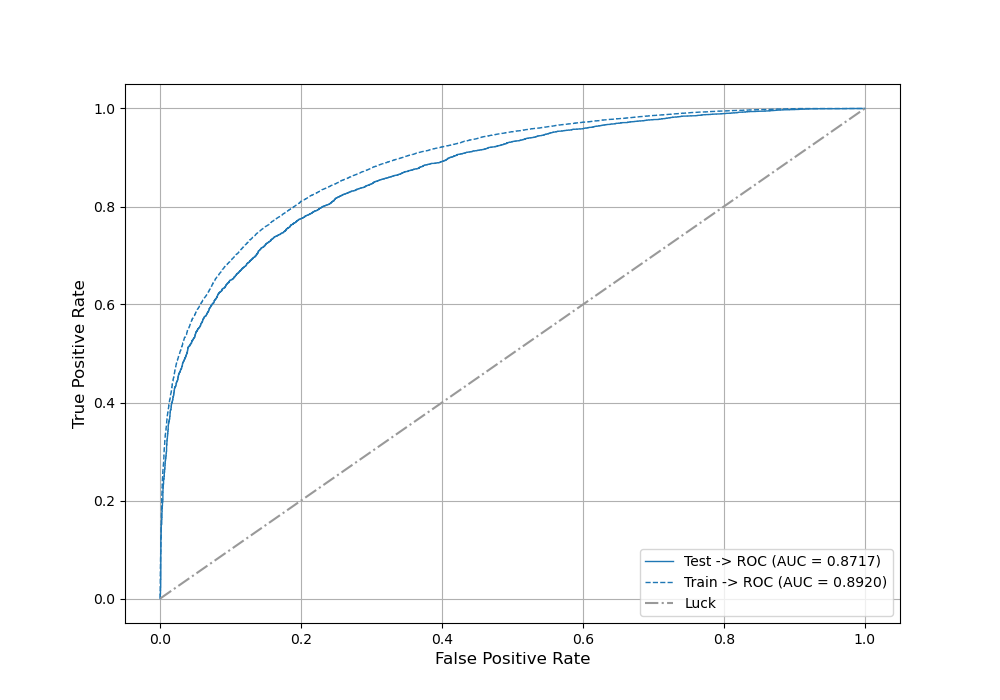
\includegraphics[width=0.5\linewidth]{gallery/results/roc_train_test_without_bkg.png}
    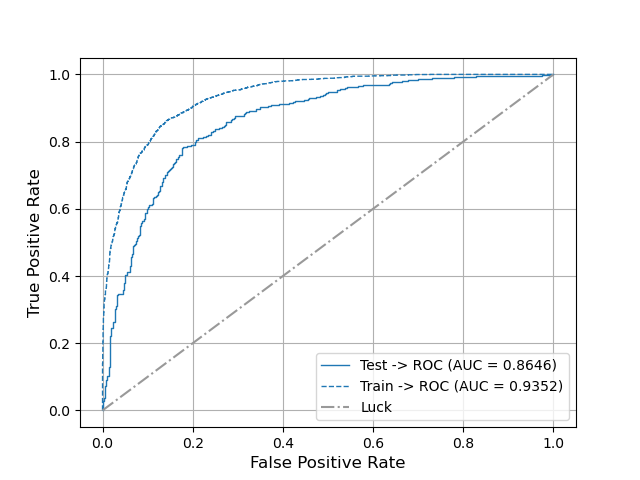
\includegraphics[width=0.46\linewidth]{gallery/results/roc_train_test_with_bkg.png}
    \caption{ROC curves for training (dashed line) vs. test data (solid line). The left plot shows results for samples without machine-background effects (Test ${\rm AUC}=0.8717$, Train ${\rm AUC}=0.8920$), and the right plot shows results for samples \textbf{with} machine-background effects (Test ${\rm AUC}=0.8646$, Train ${\rm AUC}=0.9352$).}
    \label{f.bkg_study_roc}
\end{figure}
%
Fig. \ref{f.bkg_study_roc} compares the ROC curves of the BDT models for the two data samples. In both cases, the ROC AUC for the training data and the testing data are well above 0.8, so both BDT models achieve good performance. However, for the samples \textbf{with} machine-background effects, there is significant discrepancy between the ROC curves of the training and testing data, which indicates overfitting.

%-------------------------
\subsection{Results for data with vs. without machine-background effects}

%
\begin{figure}[h!]
    \centering
    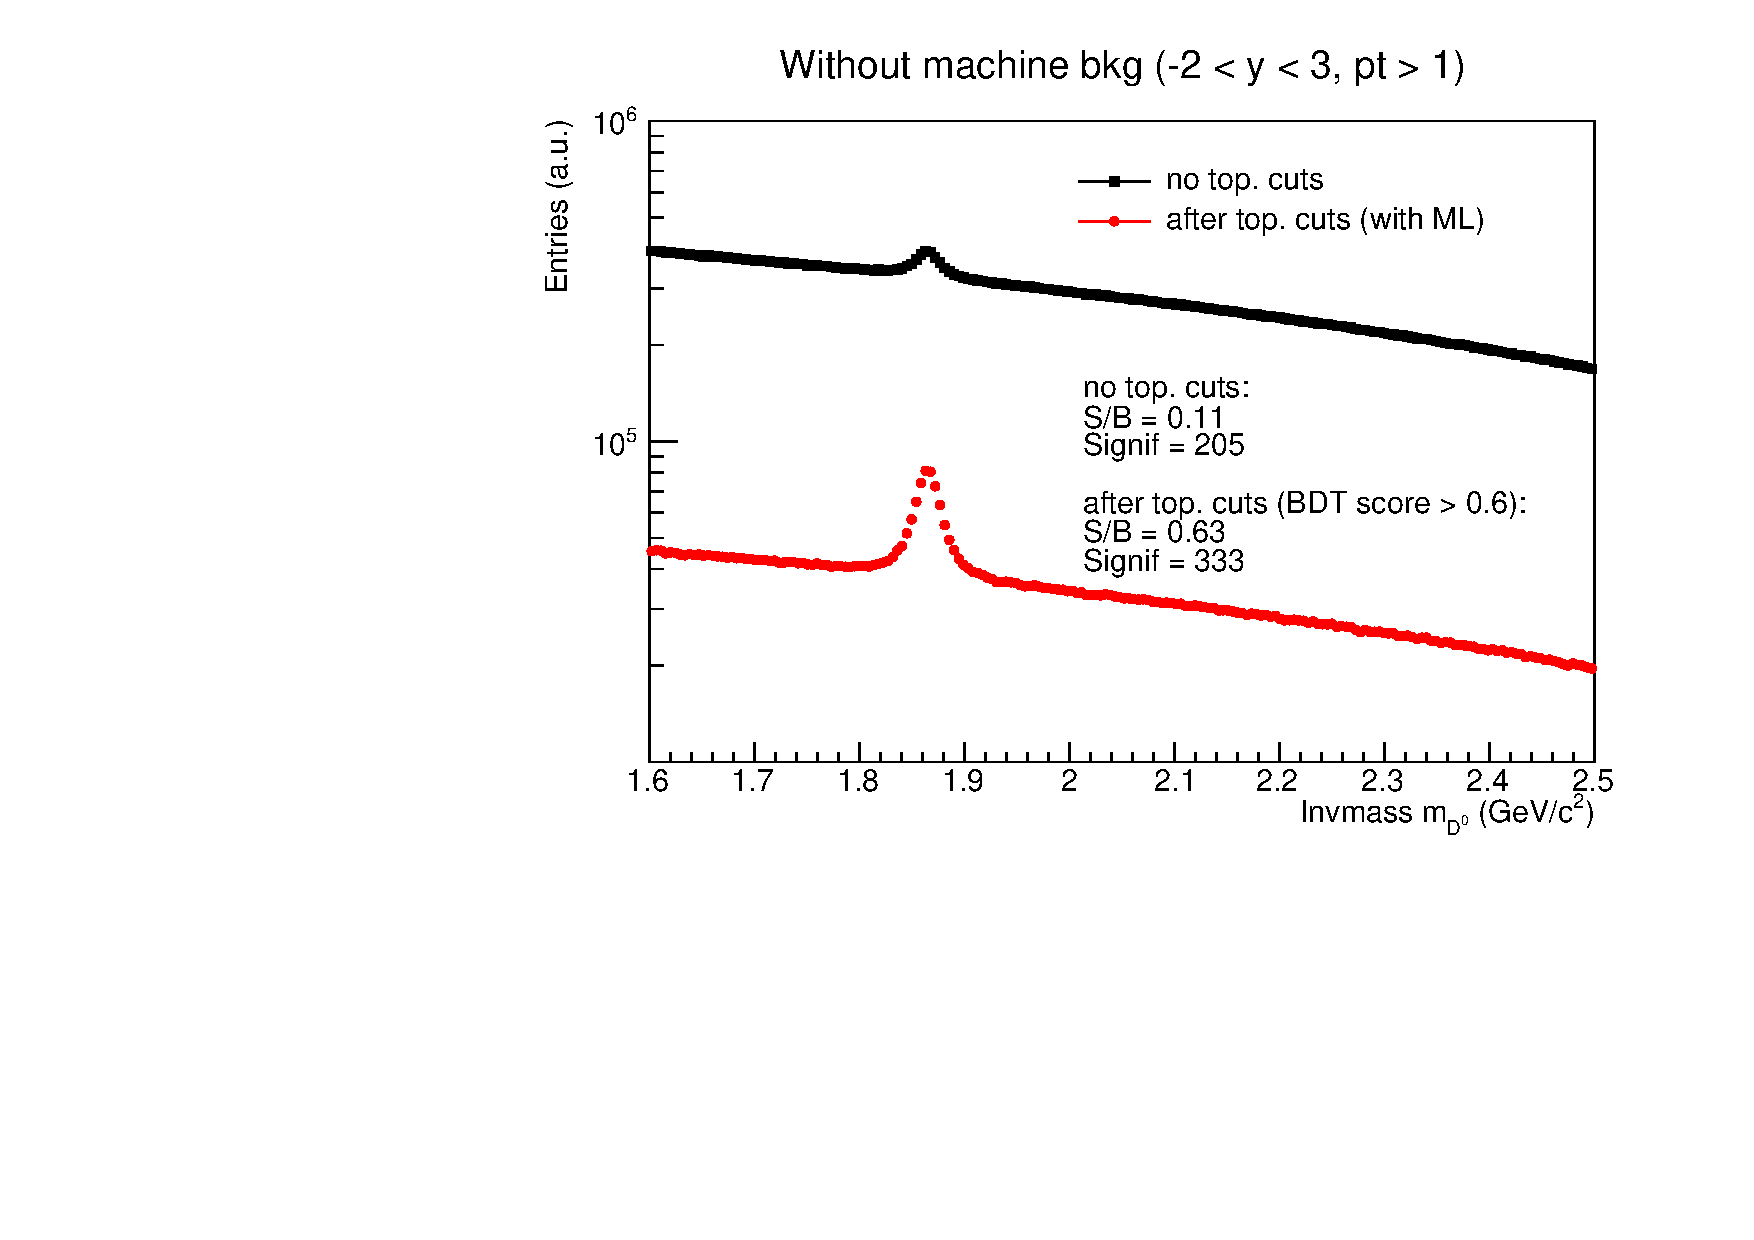
\includegraphics[width=0.6\linewidth]{gallery/results/inv_mass_without_bkg.pdf}
    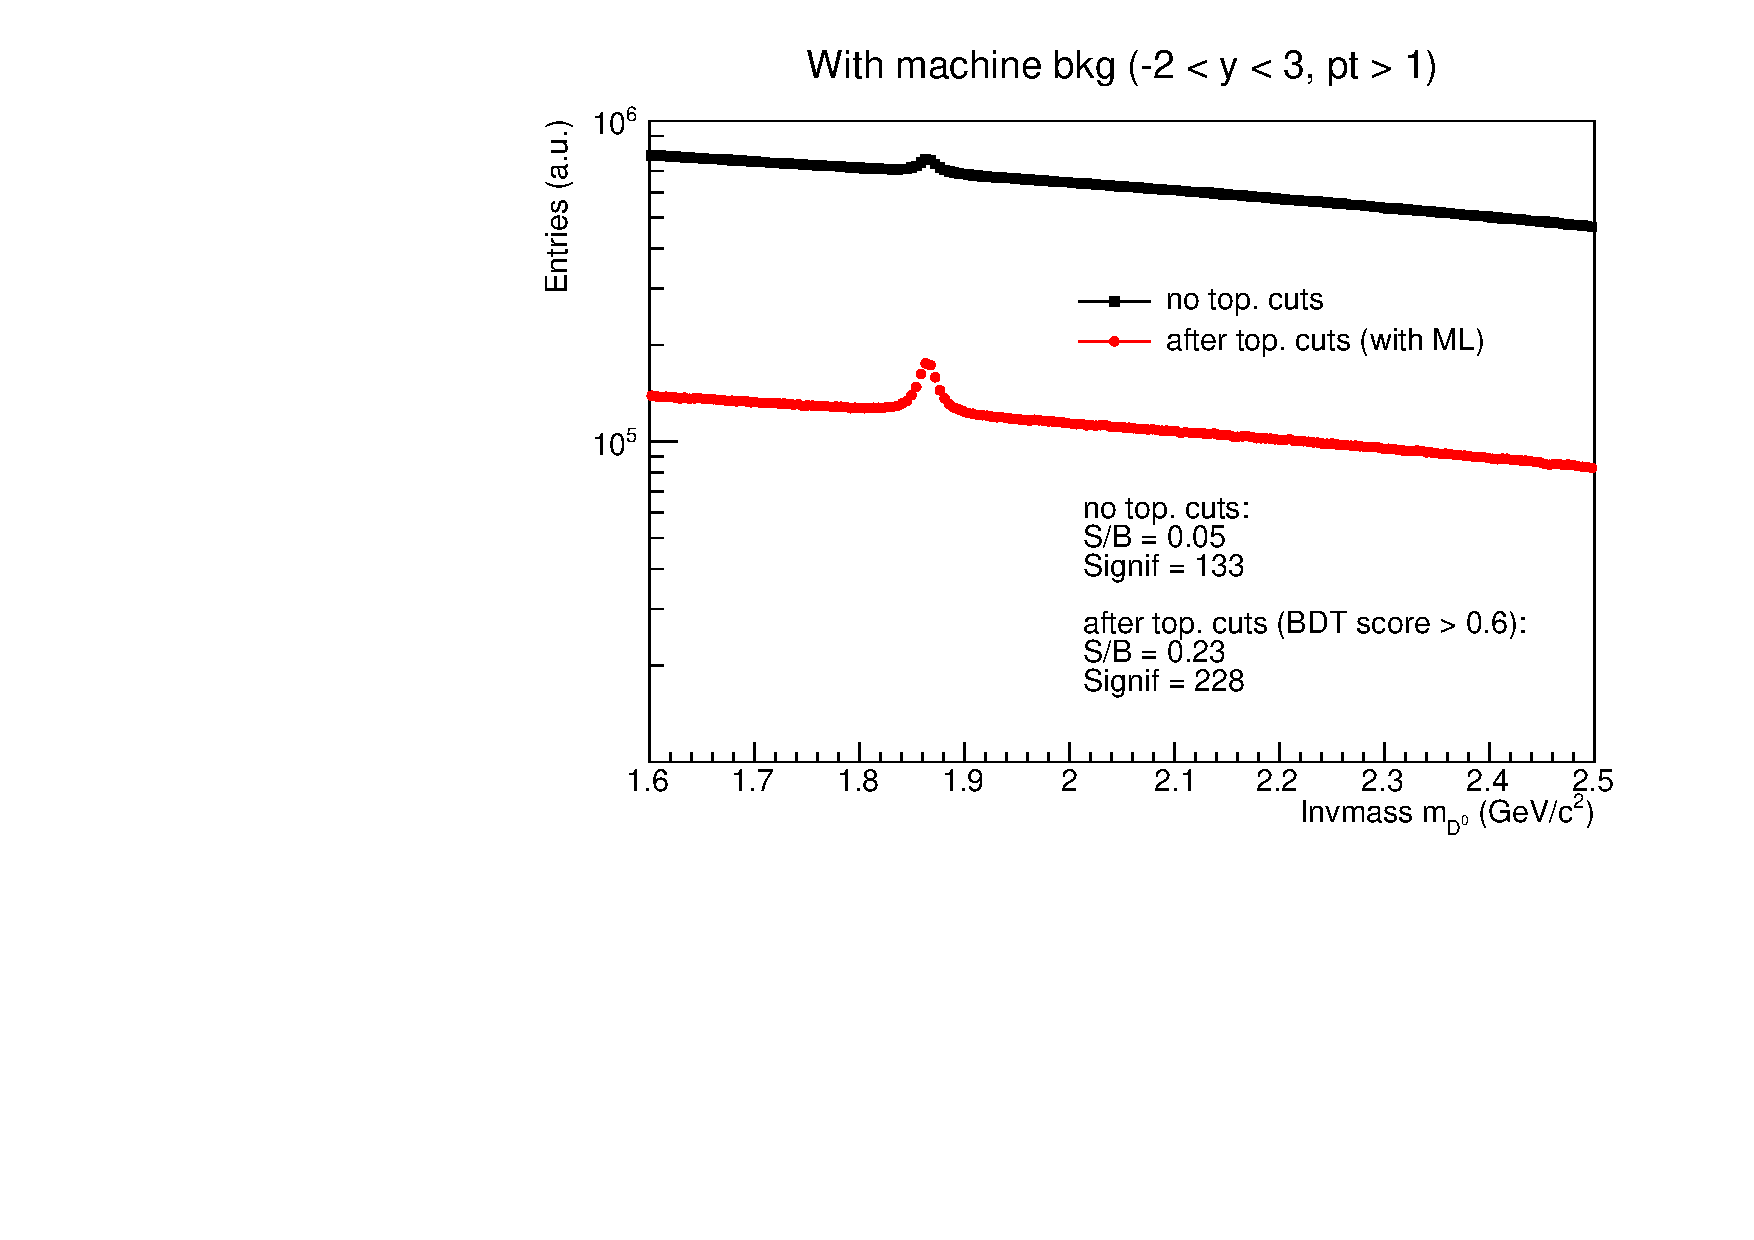
\includegraphics[width=0.6\linewidth]{gallery/results/inv_mass_with_bkg.pdf}
    \caption{Reconstructed $D^0$ invariant mass distributions before (black) vs. after (red) BDT, for samples without (top plot) and \textbf{with (bottom plot)} machine-background effects. In both samples, the plots after BDT correspond to candidates with BDT output $> 0.6$.}
    \label{f.bkg_study_inv_mass}
\end{figure}
%
Fig. \ref{f.bkg_study_inv_mass} compares the resampled invariant mass distributions before using BDT (black) and after applying BDT selections (red). We see that for both the samples \textbf{with} and without machine-background effects, applying BDT improves the S/B and Significance, with approximately a 60\% increase in Significance for the samples without machine-background effects, and a 70\% increase in Significance for the samples \textbf{with} machine-background effects. Thus, we can see more prominent $D^0$ peaks after applying BDT. Comparing the two data samples, we observe that the data \textbf{with} machine-background effects have much higher background baselines, and S/B and Significance are unfortunately much lower. This illustrates the negative impact of the machine-background effects on the efficiency with which we can reconstruct the $D^0$ invariant mass peak.

%
\begin{figure}[h!]
    \centering
    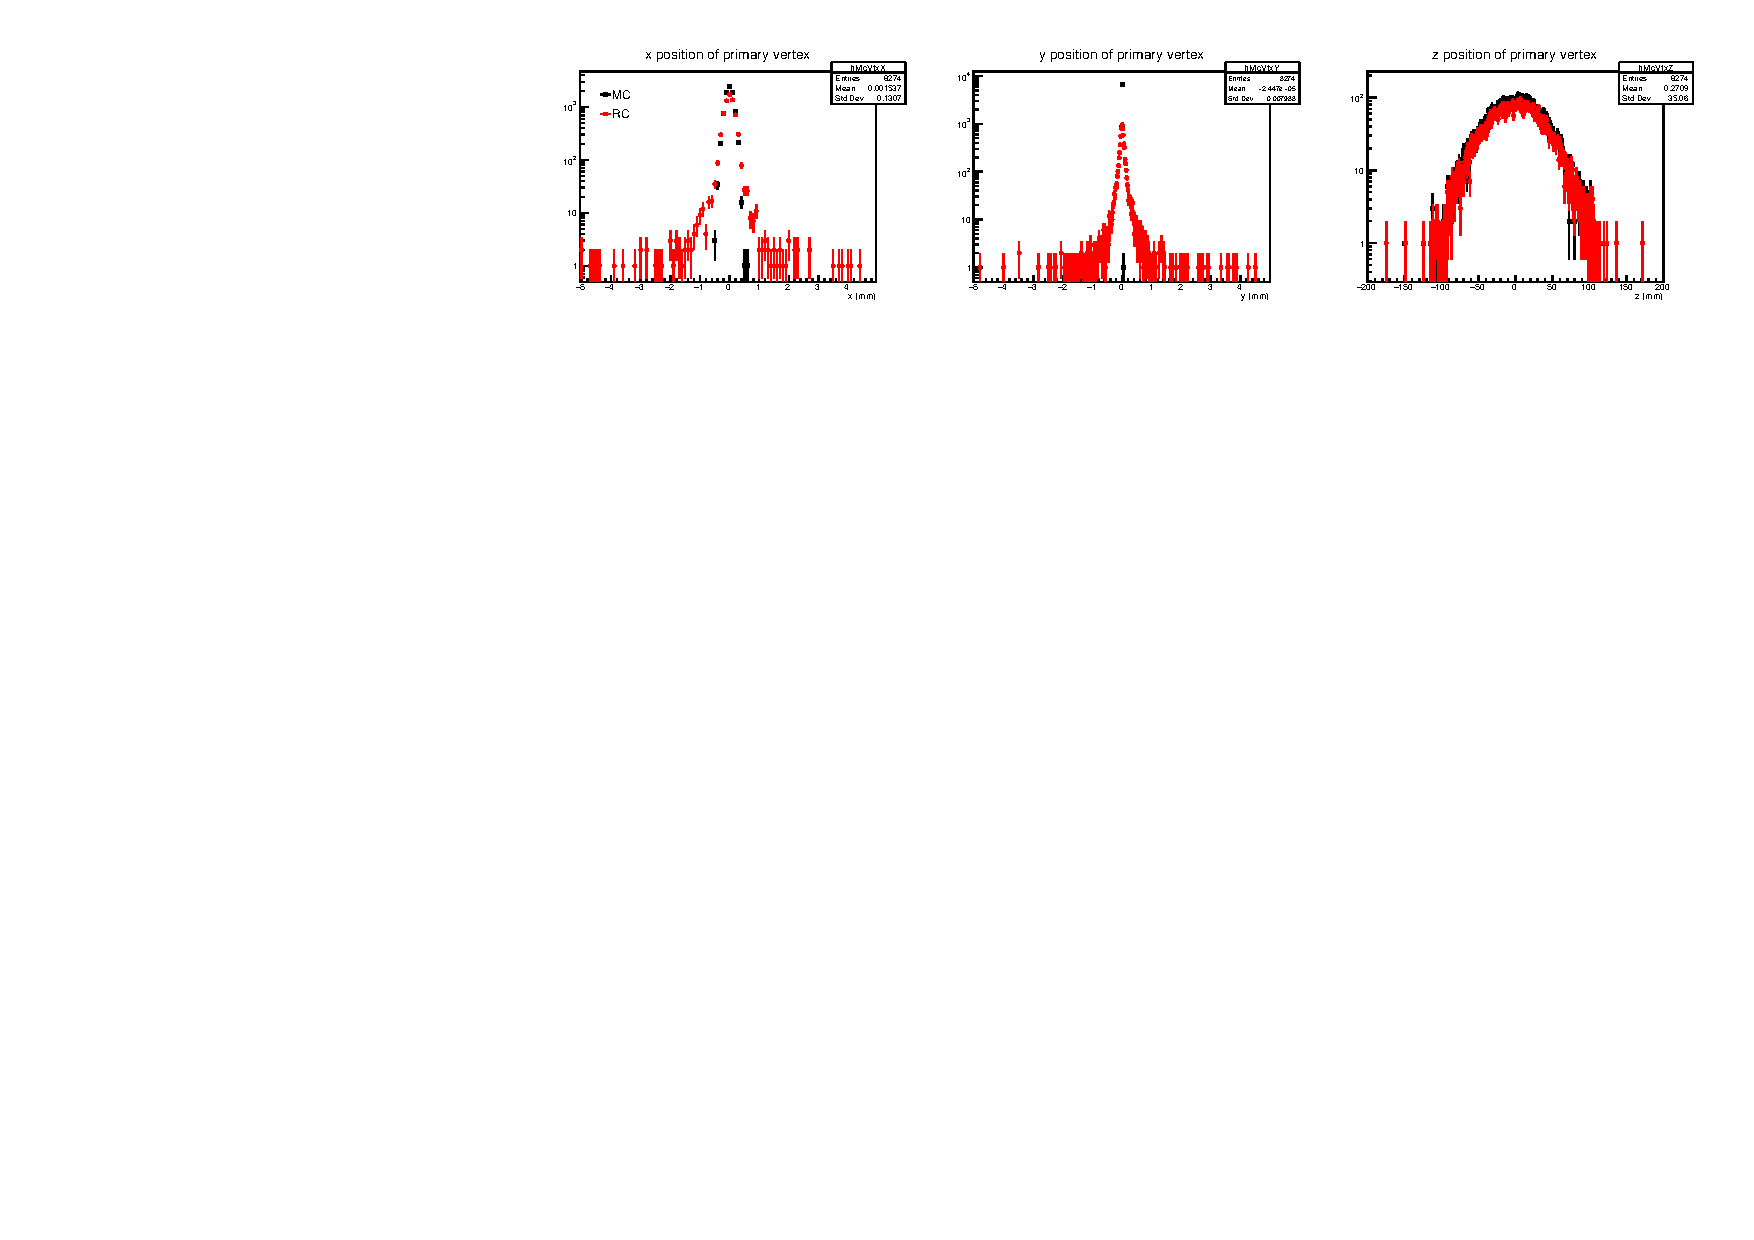
\includegraphics[width=0.95\linewidth]{gallery/results/prim_vtx_DIS_without_bkg.pdf}
    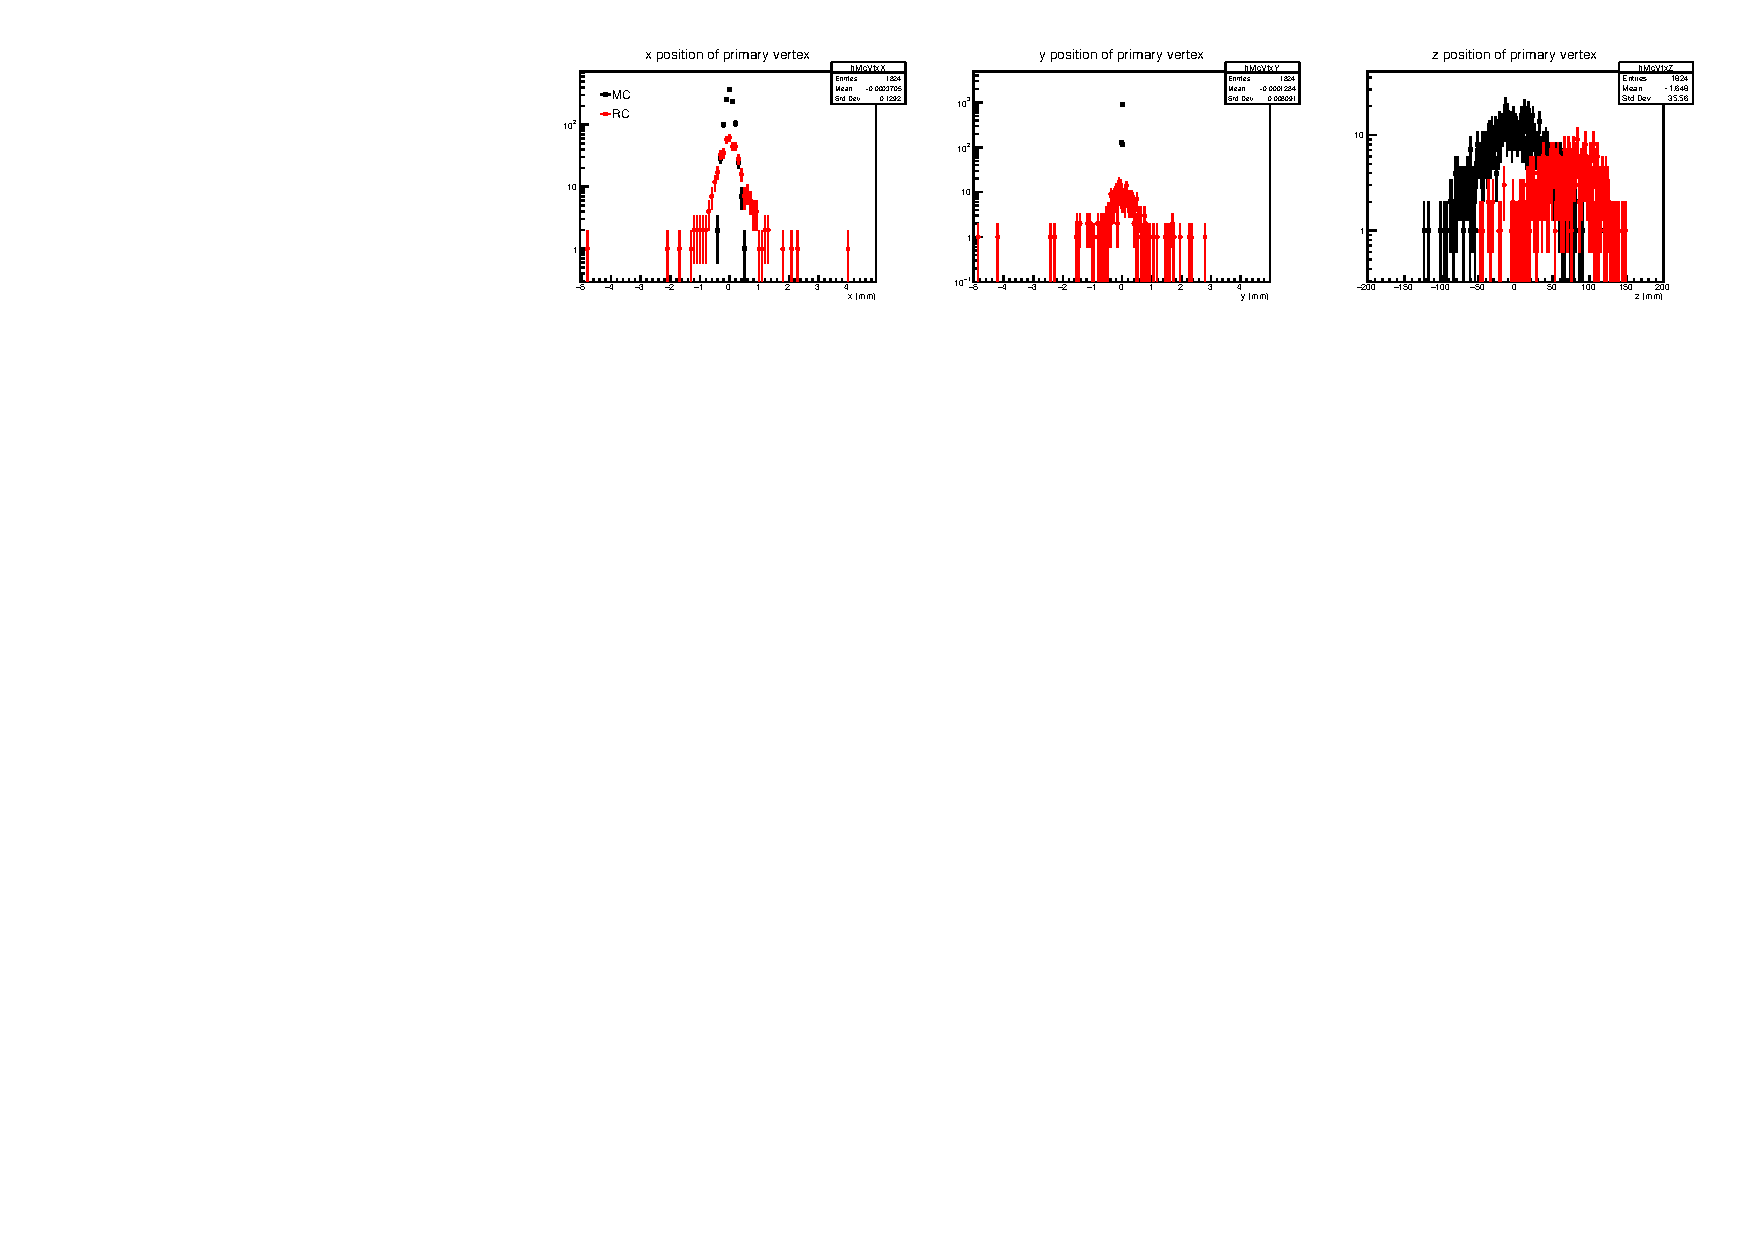
\includegraphics[width=0.95\linewidth]{gallery/results/prim_vtx_DIS_with_bkg.pdf}
    \caption{Comparisons of $x$, $y$, and $z$ locations of the reconstructed (RC) primary vertices vs. the true Monte Carlo (MC) vertices. The top shows data without machine-background effects, and the bottom shows data \textbf{with} machine-background effects.}
    \label{f.prim_vtx}
\end{figure}
%
During this study, we also found a shortcoming in the reconstruction of data \textbf{with} machine-background effects. In Fig. \ref{f.prim_vtx}, we compare the reconstructed primary vertex locations (red) to the true locations given by the Monte Carlo simulations (black). The $x$- and $y$- distributions of the reconstructed vertices are consistent with the distributions we expect from the Monte Carlo results, just with larger spreads due to reconstruction uncertainty. However, we observe that the $z$-distribution of the primary vertex for samples \textbf{with} machine-background effects (bottom right plot) is shifted off-center from the expected location. This inaccuracy of the primary vertex location leads to less reliable values for the $D^0 \rightarrow\pi+K$ topological features, which contributes to the much lower efficiency of $D^0$ signal-and-background separation. Thus, adjustments to the primary vertex reconstruction methodology is needed to improve the $D^0$ analysis.

%---------------------------------------------------------
\section{Optimizing the analysis for various slices of $y$ and $p_T$ of the $D^0$}
\label{sec.results_optimization}

To further increase the efficiency of $D^0$ signal-and-background separation, we aim to improve upon the preliminary BDT methodology (described in Ch. \ref{sec.results_prelim_methods}) in three ways:
\begin{enumerate}
    \item Analyzing the data in slices of $y$ and $p_T$, and optimizing the BDT threshold for each slice
    \item Determining the most effective combination of topological features
    \item Tuning BDT hyperparameters to adjust the model structure
\end{enumerate}
We address each of these aspects in this section.

%---------------------------
\subsection{Preliminary results in various $y$ and $p_T$ slices}
\label{sec.results_prelim}

In Ch. \ref{ch:d0_top}, we established that the $D^0\rightarrow\pi+K$ topology depends on the $y$ and $p_T$ of the $D^0$. Thus, we move forward with the analysis by dividing the data into different kinematic slices (Table \ref{tab.kinematics}):

\begin{center}
\begin{tabular}{c|c|c}
            & $-1<y<1$ & $1<y<3$ \\
            \hline
$1<p_T<2~{\rm GeV/c}$   & mid-$y$, low $p_T$ & forward $y$, low $p_T$ \\
$2<p_T<3~{\rm GeV/c}$   & mid-$y$, high $p_T$ & forward $y$, high $p_T$ \\
\end{tabular}
\end{center}

For each slice, we train a separate BDT model and optimize the BDT threshold by selecting the value that yields the highest Significance. (Here, we continue to use the same topological features and BDT hyperparameters as in the preliminary analysis.) Fig. \ref{f.inv_mass_slices} shows the $D^0$ invariant mass distributions obtained for each slice.

%
\begin{figure}[h!]
    \centering
    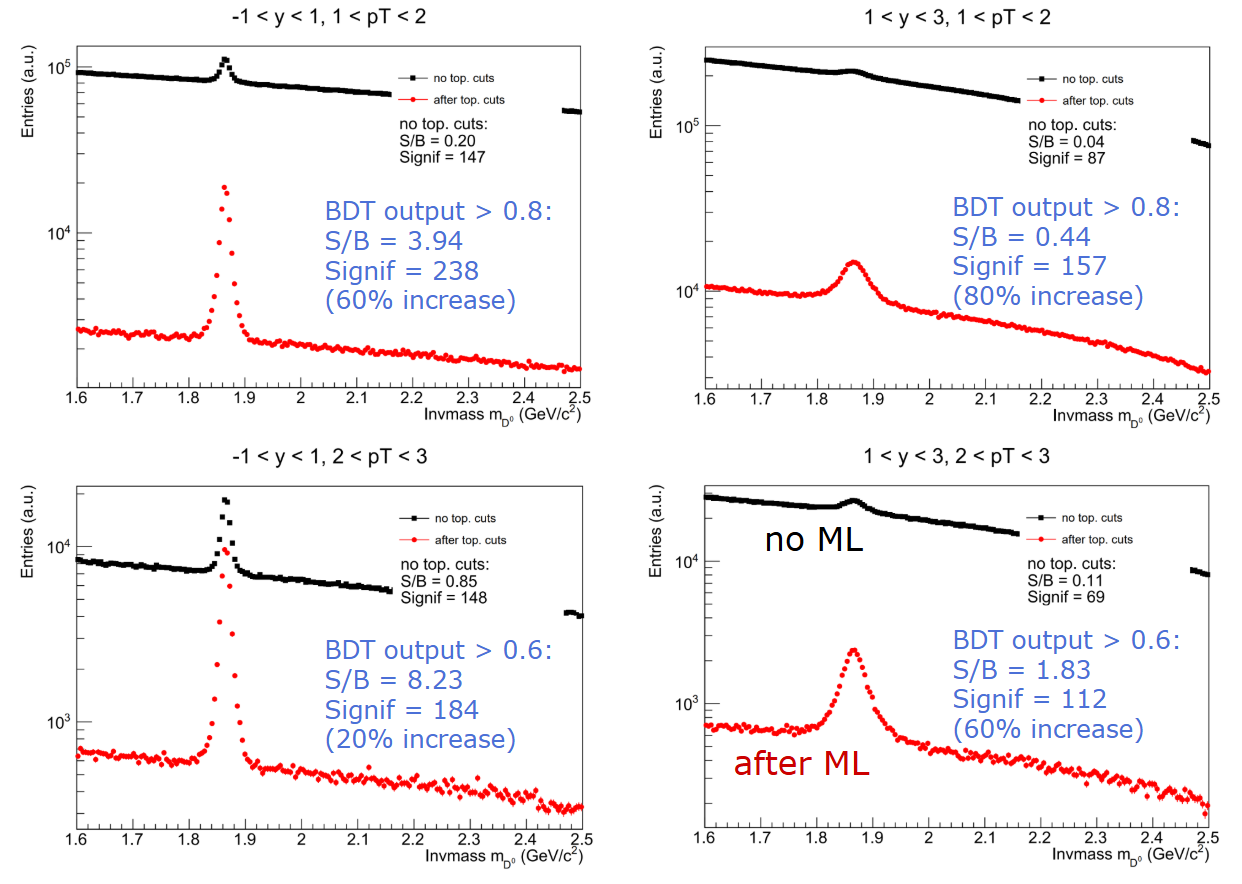
\includegraphics[width=0.9\linewidth]{gallery/results2/inv_mass_slices.png}
    \caption{Reconstructed $D^0$ invariant mass distributions before (black) vs. after (red) BDT, in various slices of $y$ and $p_T$ of the $D^0$. The BDT threshold for each slice is chosen to give the highest Significance. The \% increase denotes the change in Significance from before BDT to after BDT.}
    \label{f.inv_mass_slices}
\end{figure}
%
We observe that the resolution of the $D^0$ peak differs in each of the four slices, and the improvement in results after applying BDT also varies. Comparing low $p_T$ vs. high $p_T$ for the same $y$ range (top row vs. bottom row), we find that the high $p_T$ slice yields a higher S/B and lower Significance. This can be explained by the reconstruction of the $D^0\rightarrow \pi+K$ decay being more accurate for high $p_T$ particles, but the statistics being much lower at high $p_T$. These factors result in cleaner signal-and-background separation but larger statistical uncertainties. Comparing mid-$y$ vs. forward $y$ for the same $p_T$ range (left column vs. right column), we find that the forward $y$ yields markedly lower values of S/B and Significance. This is due to the much lower reconstruction efficiency and higher background levels in this region.

Finally, comparing the results before BDT vs. after BDT, we find that the slice which starts with the best S/B before BDT, the mid-$y$ and high $p_T$ slice (bottom left), experiences the smallest improvement after BDT, with only a 20\% increase in the Significance. Conversely, the slice with the lowest S/B before BDT, the forward $y$ and low $p_T$ slice (top right), experiences the greatest improvement after BDT, with an 80\% increase in Significance. These results indicate the BDT has the most potential for impact for this kinematic region in which the reconstruction is most difficult.

%---------------------------
\subsection{Testing various feature selections}
\label{sec.results_features}

For each kinematic slice, we then tested different combinations of topological features. In total, there are 13 features available (see Fig. \ref{f.d0_decay_diagram_2}):
\begin{multicols}{2}
\begin{itemize}
    \item \texttt{costheta}: $\cos{\theta}$
    \item \texttt{costheta\_xy}: $\cos{\theta_{xy}}$
    \item \texttt{decay\_length}: Decay Length
    \item \texttt{dca\_D0}: ${\rm DCA_{D0}}$
    \item \texttt{d0\_pi}: ${\rm DCA_\pi}$
    \item \texttt{d0xy\_pi}: ${\rm DCA}_{{\rm\pi}(xy)}$
    \item \texttt{signif\_d0xy\_pi}: ${\rm DCA}_{{\rm\pi}(xy)}/\sigma_\pi$
    \item \texttt{d0\_k}: ${\rm DCA_K}$
    \item \texttt{d0xy\_k}: ${\rm DCA}_{{\rm K}(xy)}$
    \item \texttt{signif\_d0xy\_k}: ${\rm DCA}_{{\rm K}(xy)}/\sigma_K$
    \item \texttt{sum\_d0xy}: $\sqrt{{\rm DCA}^2_{{\rm \pi}(xy)}+{\rm DCA}^2_{{\rm K}(xy)}}$
    \item \texttt{dca\_12}: ${\rm DCA_{12}}$
    \item \texttt{sigma\_vtx}: $\sigma$ of decay vertex
\end{itemize}
\end{multicols}

We first trained a BDT using all 13 features. We then examined the average SHAP values (introduced in Ch. \ref{sec.ml_shap}) to determine the most important features, then trained another BDT using only the top 5 features. Finally, we trained an additional BDT using a selection of 9 features:
\begin{multicols}{2}
\begin{itemize}
    \item \texttt{costheta}
    \item \texttt{costheta\_xy}
    \item \texttt{decay\_length}
    \item \texttt{dca\_D0}
    \item \texttt{d0\_pi}
    \item \texttt{signif\_d0xy\_pi}
    \item \texttt{d0\_k}
    \item \texttt{signif\_d0xy\_k}
    \item \texttt{sigma\_vtx}
\end{itemize}
\end{multicols}
These are slightly different from the original 10 features used in the preliminary analysis (listed Ch. \ref{sec.results_prelim}).

%
% \begin{figure}[h!]
%     \centering
%     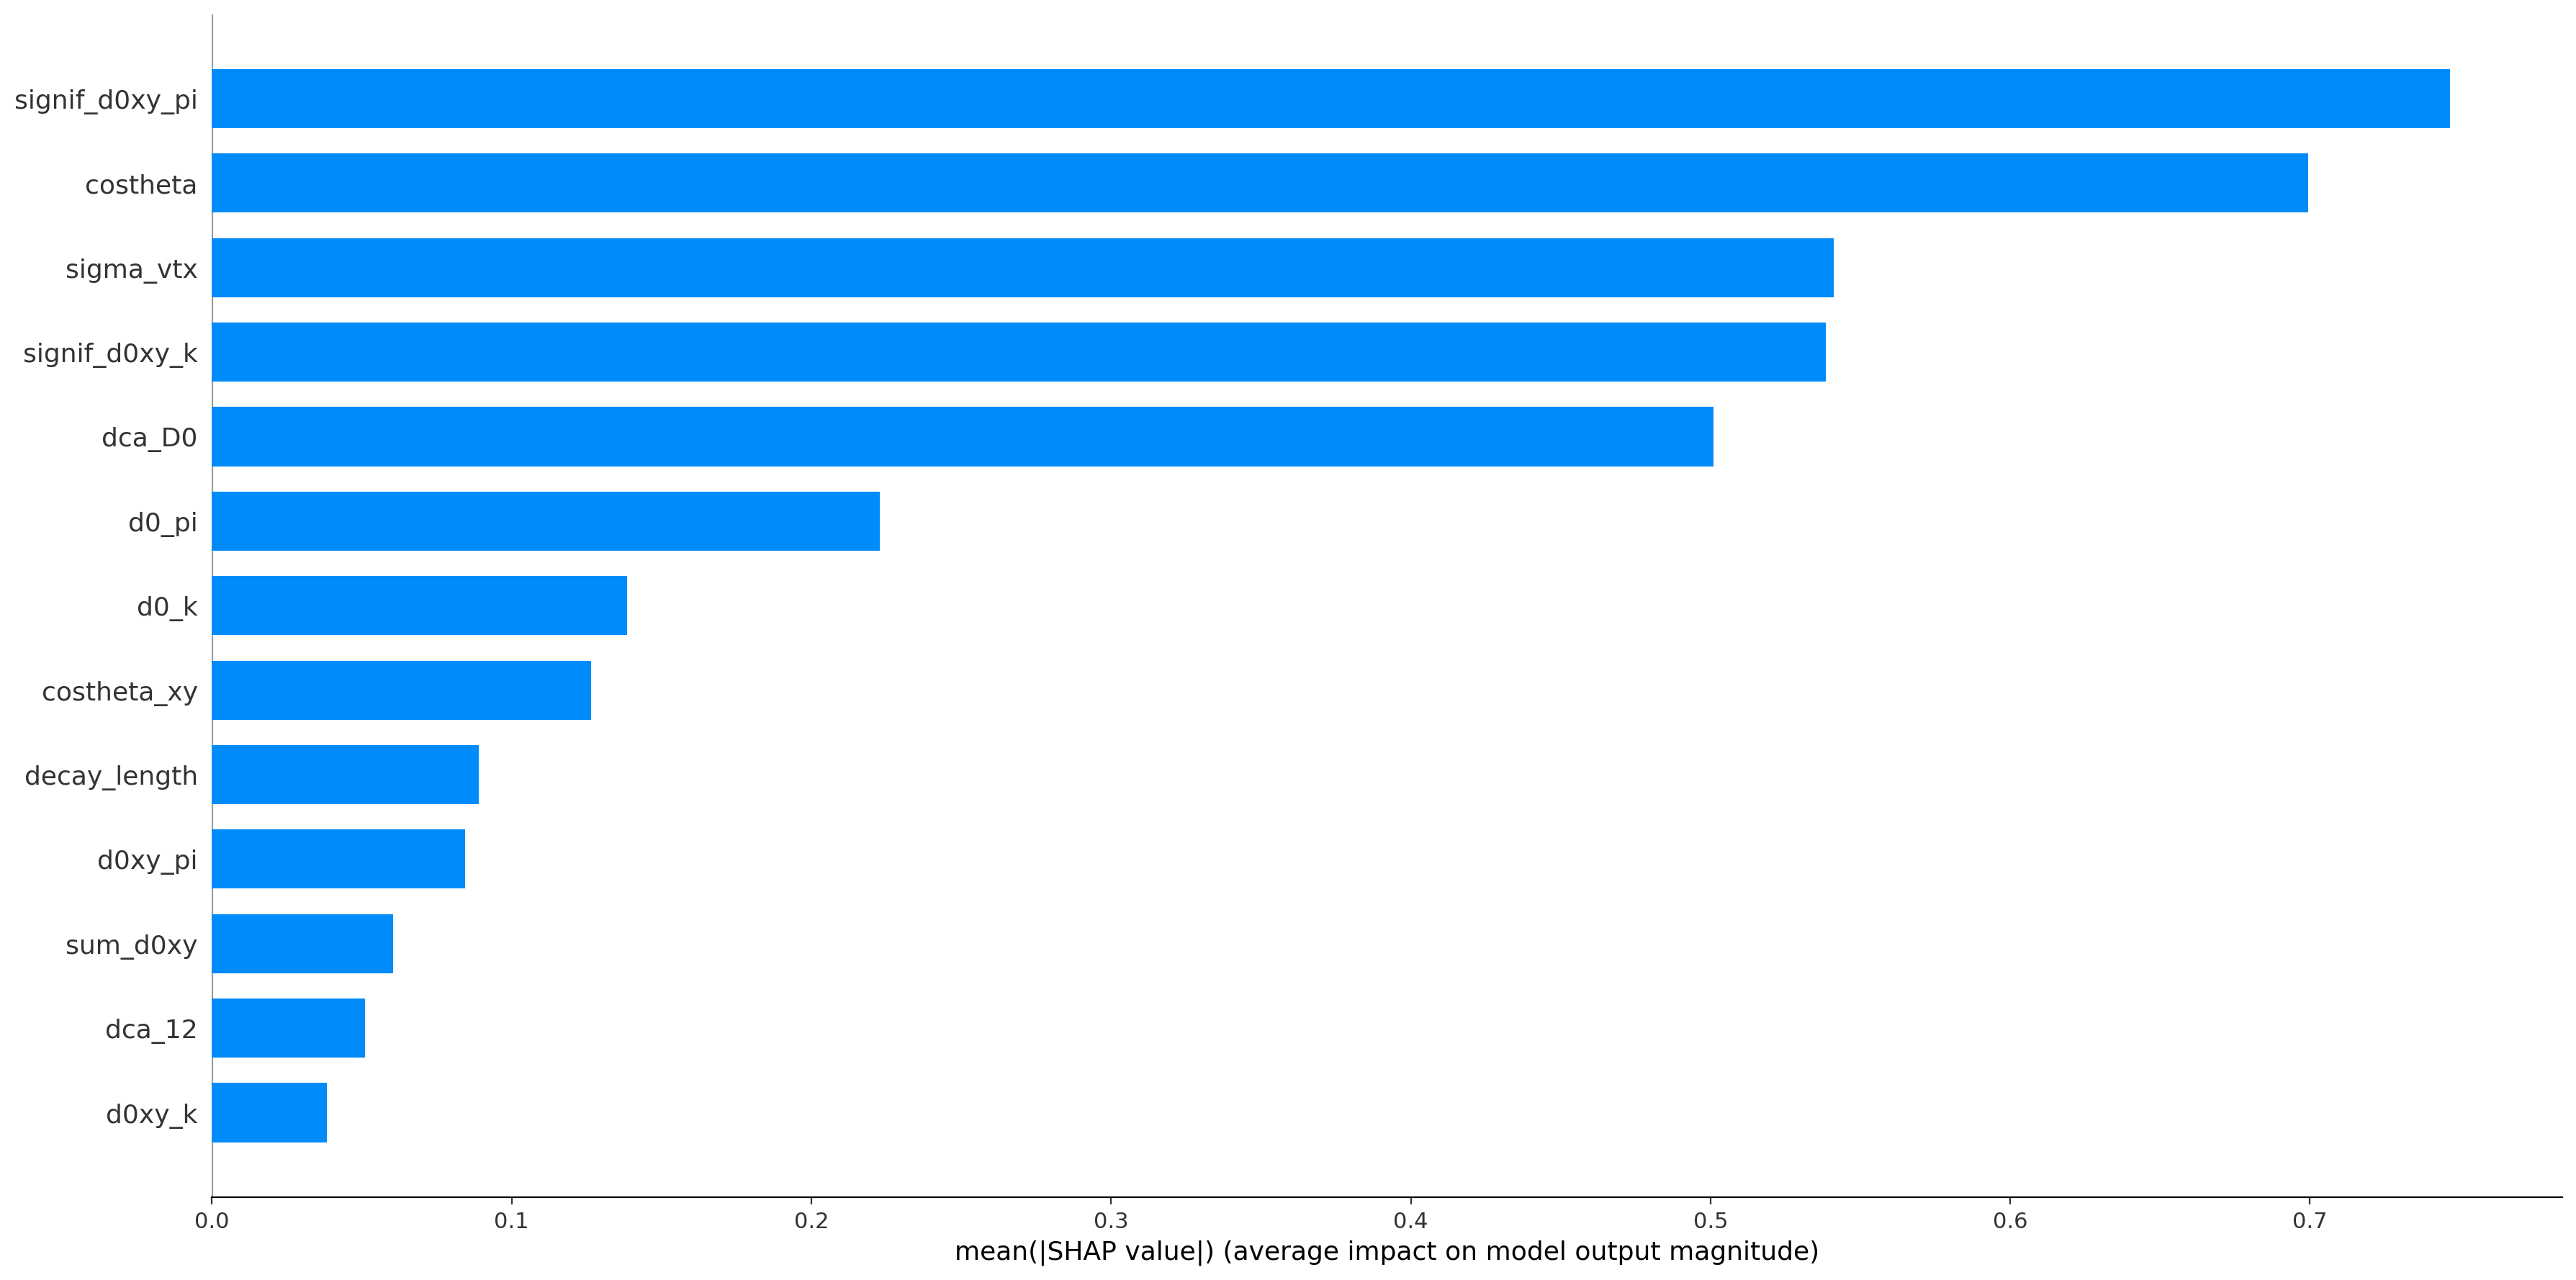
\includegraphics[width=0.95\linewidth]{gallery/results2/all_shap_feature_impact.png}
%     \caption{Average SHAP values of all 13 topological features for $1<y<3$ and $1<p_T<3$.}
%     \label{f.all_shap}
% \end{figure}
%

%
\begin{figure}[h!]
    \centering
    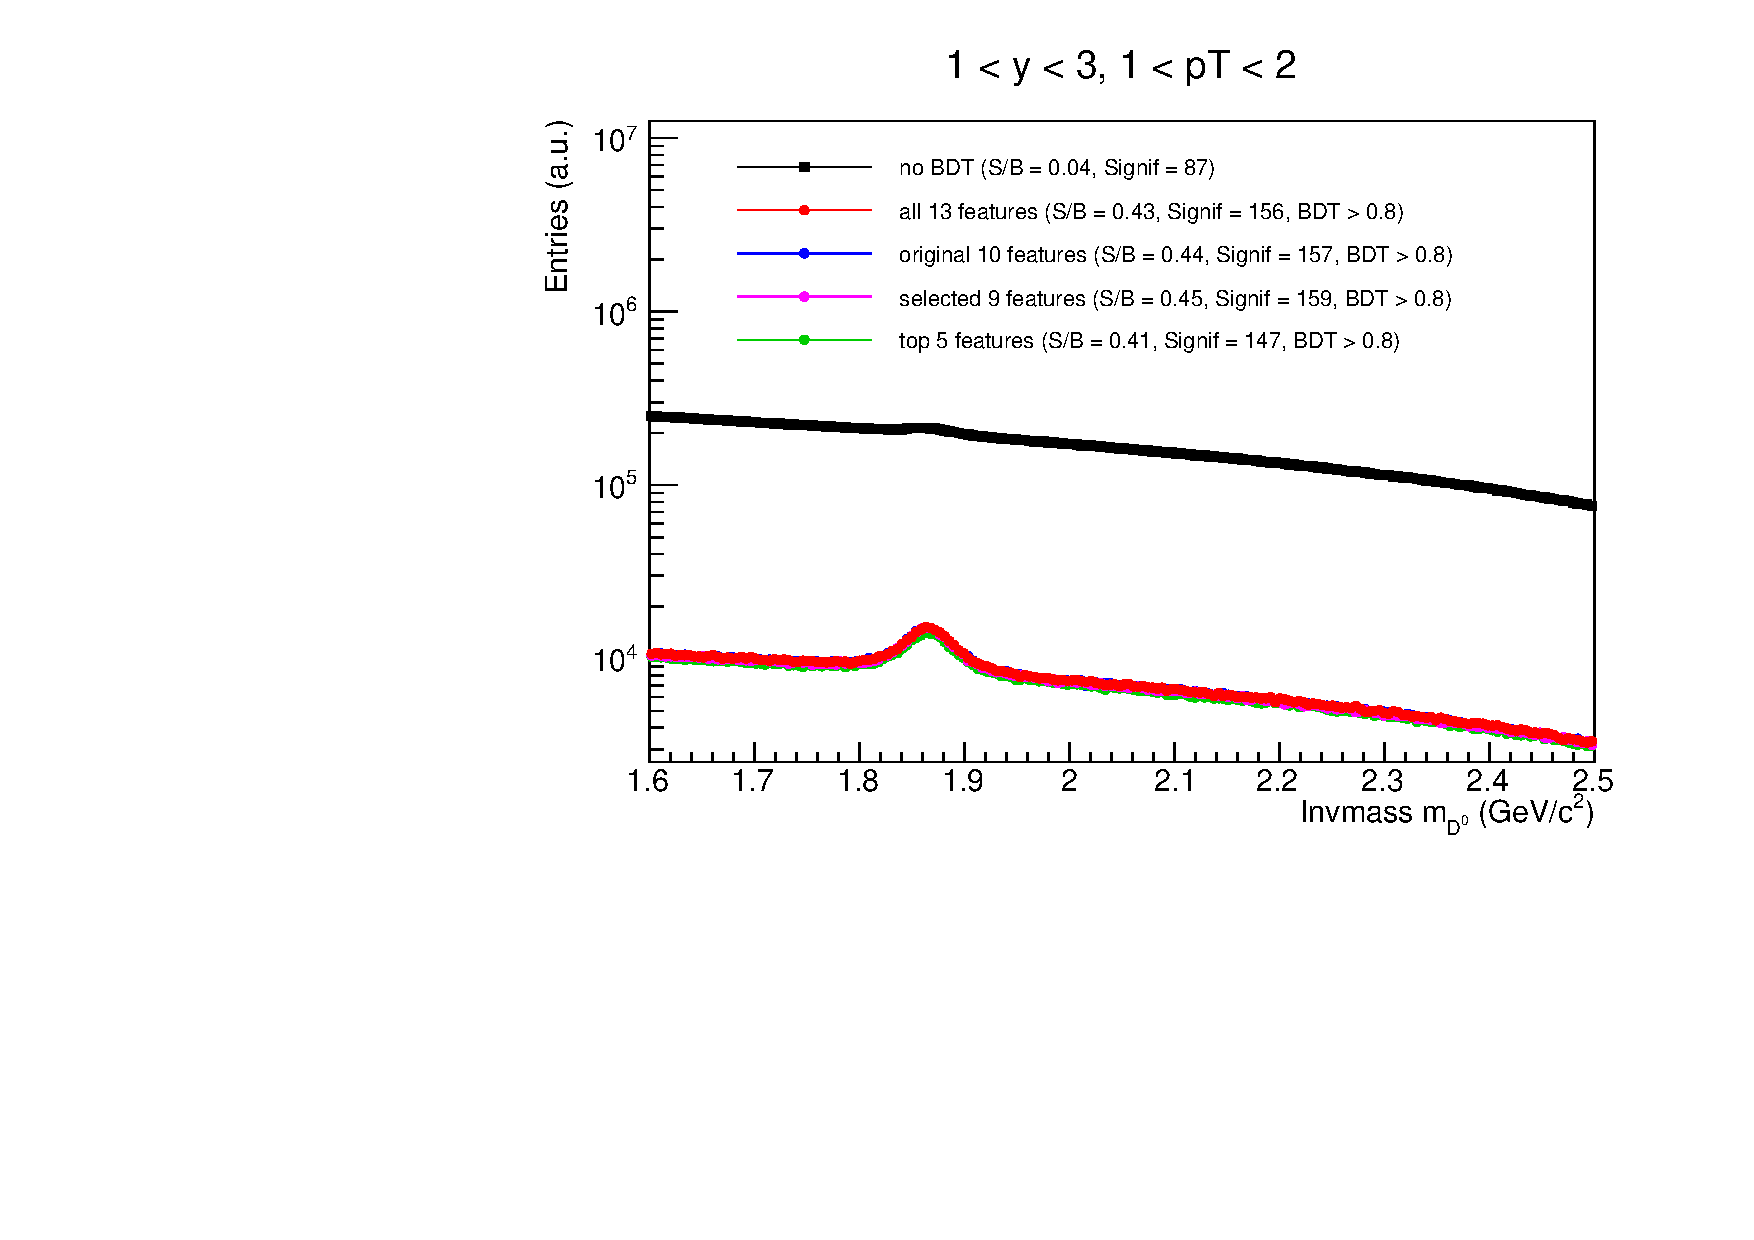
\includegraphics[width=0.65\linewidth]{gallery/results2/inv_mass_diff_features_y_1.0_3.0_pt_1.0_2.0_bdt_0.8.pdf}
    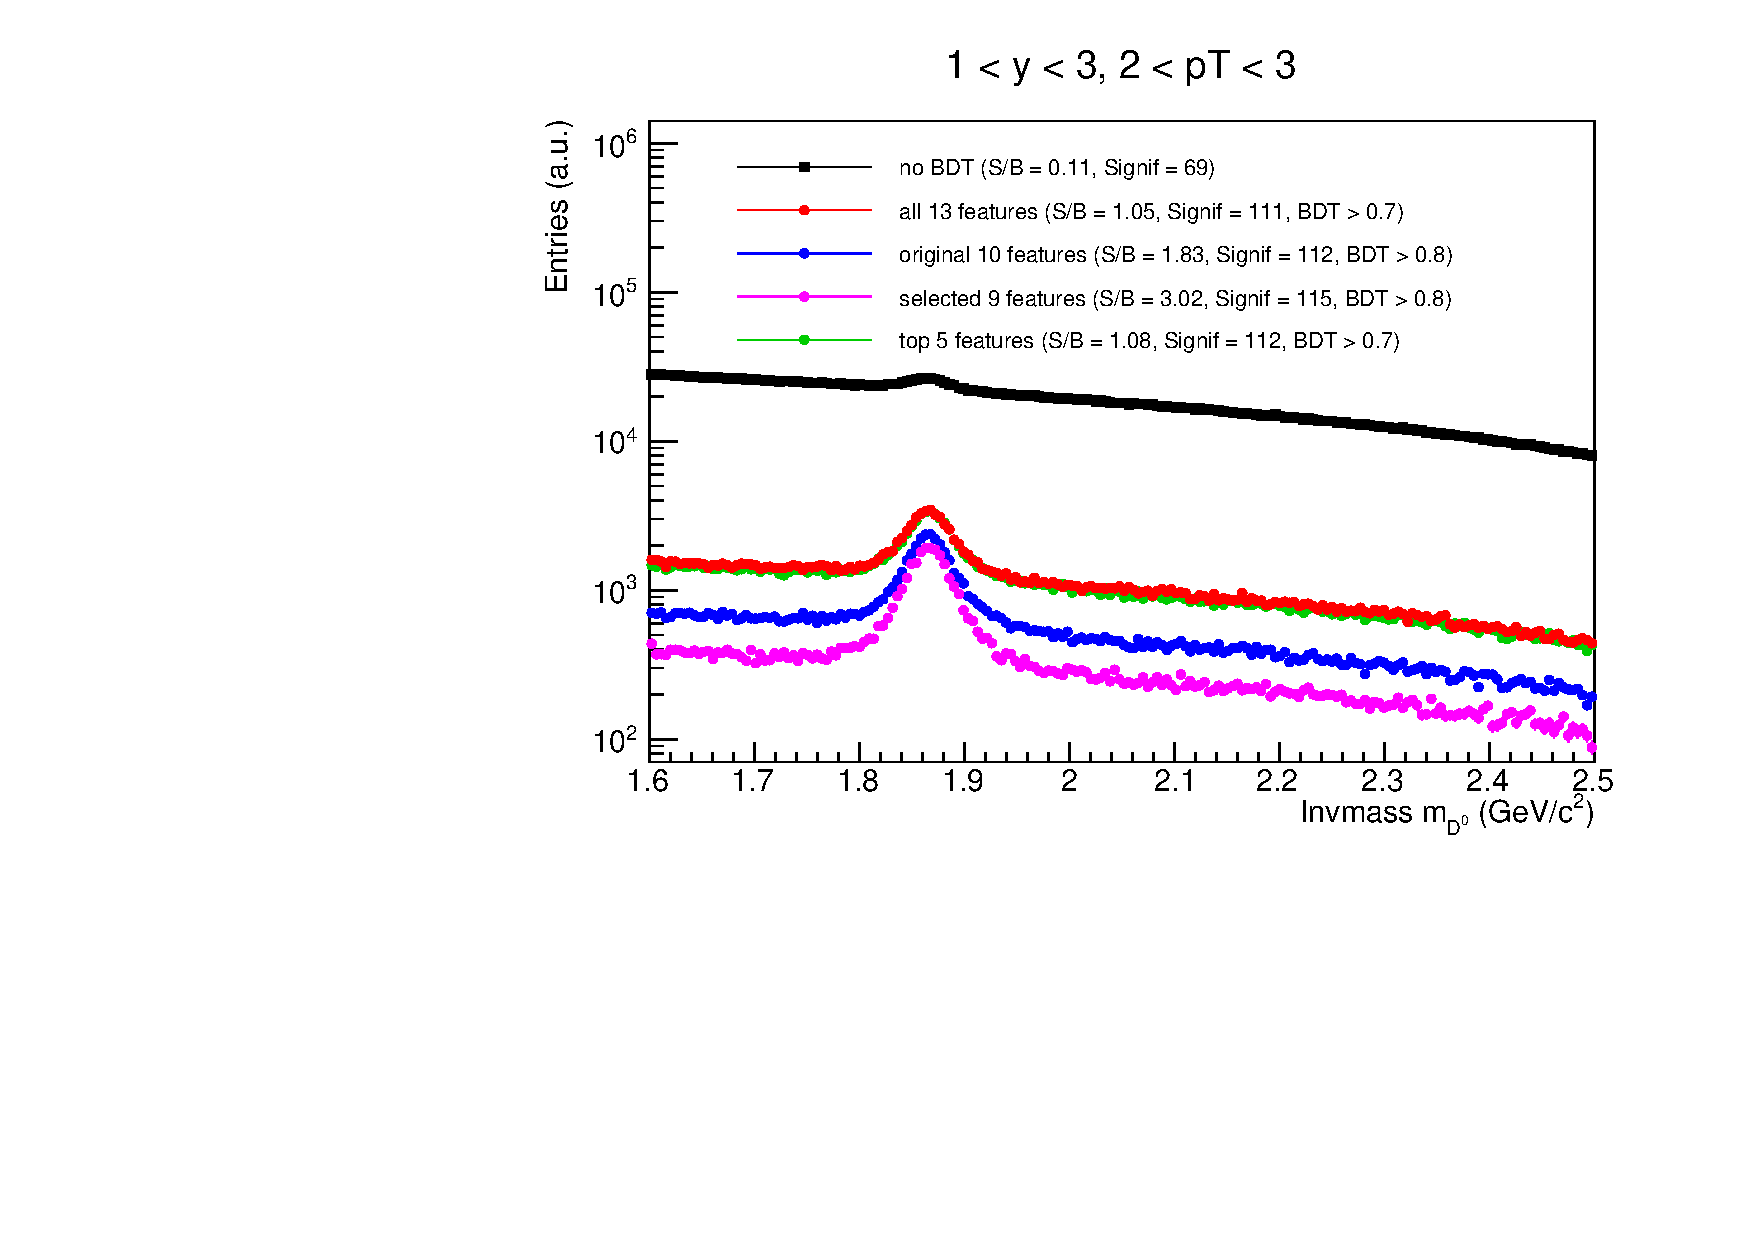
\includegraphics[width=0.65\linewidth]{gallery/results2/inv_mass_diff_features_y_1.0_3.0_pt_2.0_3.0_bdt_0.7.pdf}
    \caption{Reconstructed $D^0$ invariant mass distributions before BDT (black) vs. after applying BDTs trained using various features selections: all 13 available features (red), the original 10 preliminary features (blue), a selection of 9 features (magenta), and the top 5 most important features (green). The top plot shows data for $1<y<3$ and $1<p_T<2~{\rm GeV/c}$, and the bottom plot shows data for $1<y<3$ and $2<p_T<3~{\rm GeV/c}$. Each BDT threshold is selected to yield the highest Significance.}
    \label{f.feature_selections}
\end{figure}
%
Fig. \ref{f.feature_selections} shows examples of the resulting $D^0$ invariant mass distributions obtained using BDTs trained with these various feature combinations. For the forward $y$ and high $p_T$ slice (top plot), we observe that all these different feature selections produce the same results. However, for the high $p_T$ slice (bottom plot), we do notice an impact of feature selection. In particular, the BDT trained using the selection of 9 features (magenta) yields the highest S/B and Significance, thus distinguishing this selection to be the best combination of features for this kinematic slice. The BDT trained using the original 10 features (blue) yields the second best results. Interestingly, the BDT trained using all 13 available features (red) and that trained using only the top 5 features (green) both produce similar results, which are worse than the other two models.

From these results, we can conclude that simply including more features will not necessarily improve BDT performance. This is perhaps unsurprising, as once the most important features are included, any additional features will only produce a small impact on the BDT outputs. Thus, in some instances, the best choice of features is somewhat arbitrary. This is more likely the case for kinematic regions with high statistics, in which the BDT has a sufficiently large training dataset to learn the true signal-and-background boundaries (provided that a few of the most important features are included).

However, the results for the high $p_T$ slice also demonstrate that BDT performance can sometimes worsen as more features are added. This issue tends to arise in such regions with lower statistics, in which the data contains more statistical fluctuations and the BDT is thus more sensitive to feature selection. This might be because providing the BDT with a large number of features gives the model too much flexibility in fitting the training data, which increases the likelihood of overfitting and thus leads to worse performance on testing data. Kinematic regions with high statistics are generally more robust to this issue.

% We can find some explanation for this observation in the BDT output distributions of Fig. \ref{f.bdt_all_vs_fav}, comparing the model trained using the selected 9 features and the model trained using all 13 features.
% %
% \begin{figure}[h!]
%     \centering
%     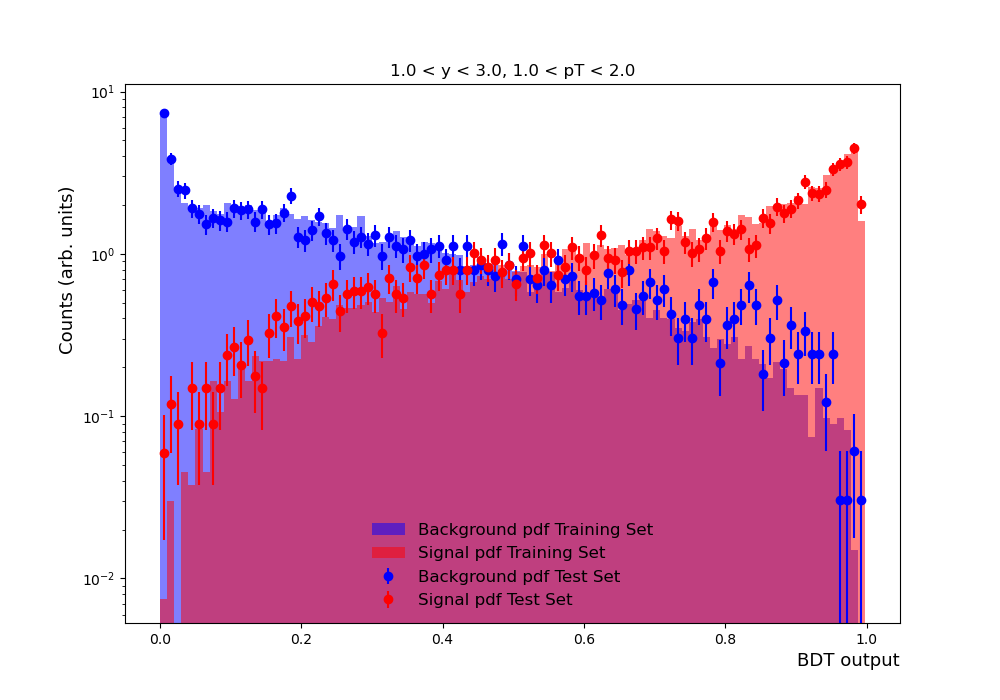
\includegraphics[width=0.45\linewidth]{gallery/results2/fav_train_test.png}
%     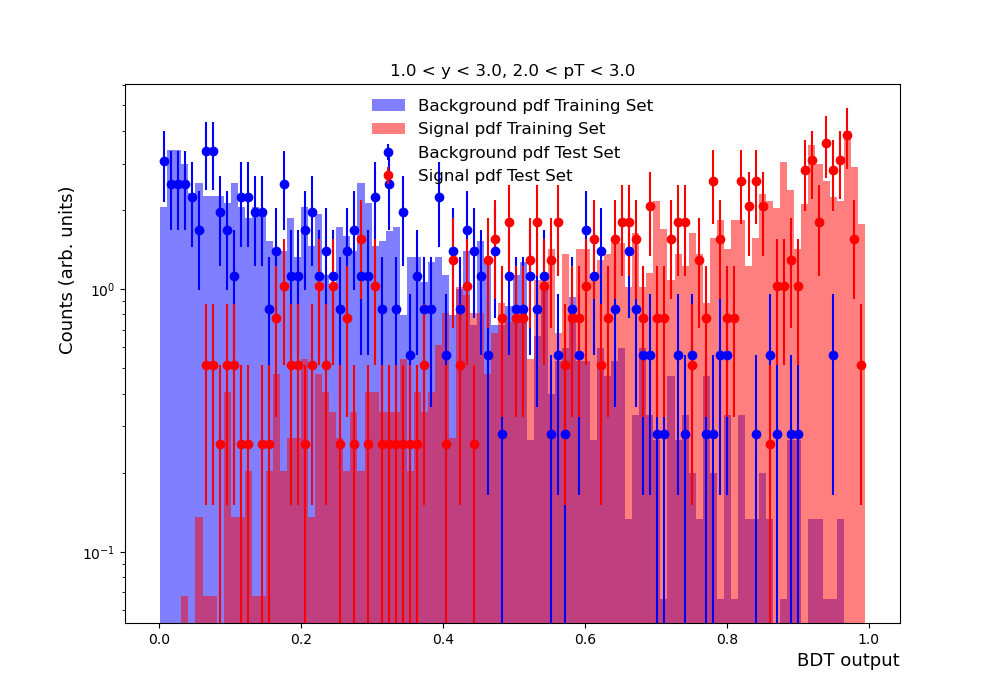
\includegraphics[width=0.45\linewidth]{gallery/results2/all_train_test.png}
%     \caption{BDT output distributions for training and testing data in $1<y<3$ and $2<p_T<3~{\rm GeV/c}$. The left plot shows results for a BDT trained using the selected 9 features, and the right plot shows results for a BDT trained using all 13 features.}
%     \label{f.bdt_all_vs_fav}
% \end{figure}
% %
% In Fig. \ref{f.bdt_all_vs_fav}, we observe that the BDT with 13 features (right plot) exhibits much flatter output distributions, which indicates a less clearly delineated separation between signal and background candidates. {\color{brown} What else to say about this? How to interpret and explain the worse performance???}

%
\begin{figure}[h!]
    \centering
    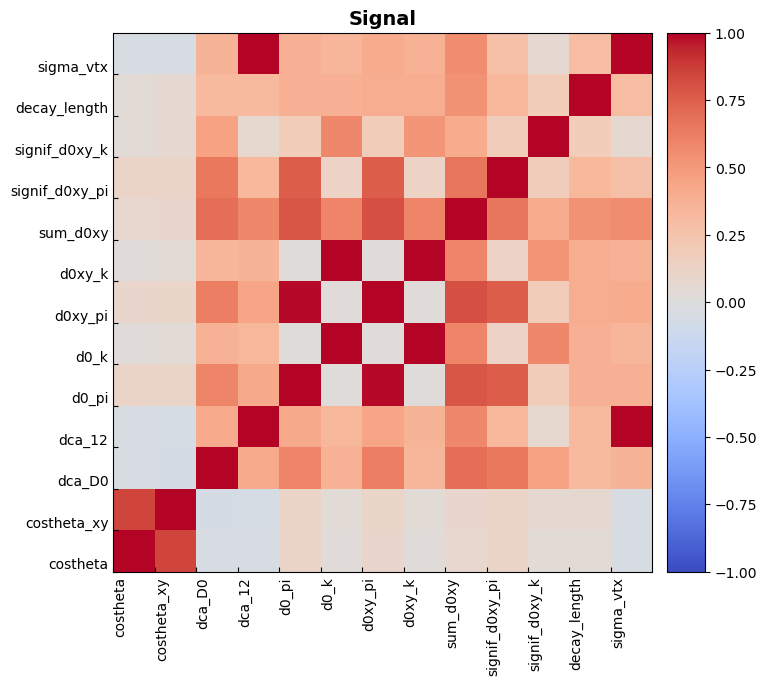
\includegraphics[width=0.8\linewidth]{gallery/results2/all_correlation_plot_sig.png}
    \caption{Correlation coefficients of all 13 topological features, for signal candidates in $1<y<3$ and $2<p_T<3~{\rm GeV/c}$. A value of 1 (dark red) indicates perfect positive correlation, and a value of -1 (dark blue) indicates perfect negative correlation.}
    \label{f.all_corr}
\end{figure}
%
Fig. \ref{f.all_corr} shows the correlations between these features. As expected, features defined with respect to one another---\texttt{costheta} and \texttt{costheta\_xy}, \texttt{dca\_12} and \texttt{sigma\_vtx}, as well as the various measurements for DCA of the pion and kaon---are positively correlated. However, our results demonstrate that BDTs are surprisingly robust to feature correlations. This makes sense given that BDTs tend to systematically favor the use of one feature over another when the two are highly correlated, and thus the models remain largely unaffected by the redundancies introduced by correlations. Nonetheless, it is generally advisable to eliminate strong correlations between features in order to improve the computational efficiency of the BDT and the interpretability of the results.

%---------------------------
\subsection{Tuning BDT hyperparameters}
\label{sec.results_hyperparams}

For the last aspect of our BDT optimization, we examine the impacts on model performance that can result from choices made during hyperparameter optimization. In our analysis, we utilize Optuna \cite{Optuna} to optimize the first five hyperparameters listed in Ch. \ref{sec.ml_optuna}. We consider \texttt{n\_estimators}, \texttt{max\_depth}, and \texttt{learning\_rate} to be the ``basic" hyperparameters, and we consider \texttt{min\_child\_weight} and \texttt{min\_split\_loss} to be less essential ``regulatory" hyperparameters.

In case I, we optimize the three basic hyperparameters, restricting them to the relatively conservative ranges:
\begin{itemize}
    \item \texttt{n\_estimators}: (100, 400)
    \item \texttt{max\_depth}: (1, 3)
    \item \texttt{learning\_rate}: (0.01, 0.1)
\end{itemize}
with all other hyperparameters set to default values. This is the same condition as in the preliminary analysis. In case II, we then expand the ranges to:
\begin{itemize}
    \item \texttt{n\_estimators}: (100, 800)
    \item \texttt{max\_depth}: (1, 8)
    \item \texttt{learning\_rate}: (0.01, 0.3)
\end{itemize}
Lastly in case III, we optimize the two regulatory hyperparameters alongside the initial three:
\begin{itemize}
    \item \texttt{n\_estimators}: (100, 800)
    \item \texttt{max\_depth}: (1, 8)
    \item \texttt{learning\_rate}: (0.01, 0.3)
    \item \texttt{min\_child\_weight}: (1, 10)
    \item \texttt{min\_split\_loss}: (0, 5)
\end{itemize}

In Table \ref{tab.optuna}, we list the best hyperparameter values determined by Optuna in each of the three cases for $1<y<3$ and $1<p_T<2~{\rm GeV/c}$. We notice that when given greater flexibility, Optuna tends to select large values for \texttt{max\_depth}. In case III, we also observe a larger value for \texttt{n\_estimators}, which reaches beyond the original range set in case I. Although in cases II and III, the values of other hyperparameters decrease to offset the increase in \texttt{max\_depth} (and \texttt{n\_estimators}), we find that these hyperparameter values result in overfitting. This can be observed in the ROC curves of Fig. \ref{f.bdt_hyperparams}, which compares the results for case I and case III.

\begin{table}[h!]
    \centering
    \begin{tabular}{l|c|c|c}
         &  Case I & Case II & Case III \\
         \hline
         \texttt{n\_estimators} & 480 & 347 & 728 \\
         \texttt{max\_depth} & 3 & 6 & 8 \\
         \texttt{learning\_rate} & 0.067 & 0.034 & 0.011 \\
         \texttt{min\_child\_weight} & 1 & 1 & 10 \\
         \texttt{min\_split\_loss} & 0 & 0 & 1
    \end{tabular}
    \caption{Best hyperparameter values selected by Optuna for the three cases examined in $1<y<3$ and $1<p_T<2~{\rm GeV/c}$. \texttt{min\_child\_weight} = 1 and \texttt{min\_split\_loss} = 0 are default values.}
    \label{tab.optuna}
\end{table}

%
\begin{figure}[h!]
    \centering
    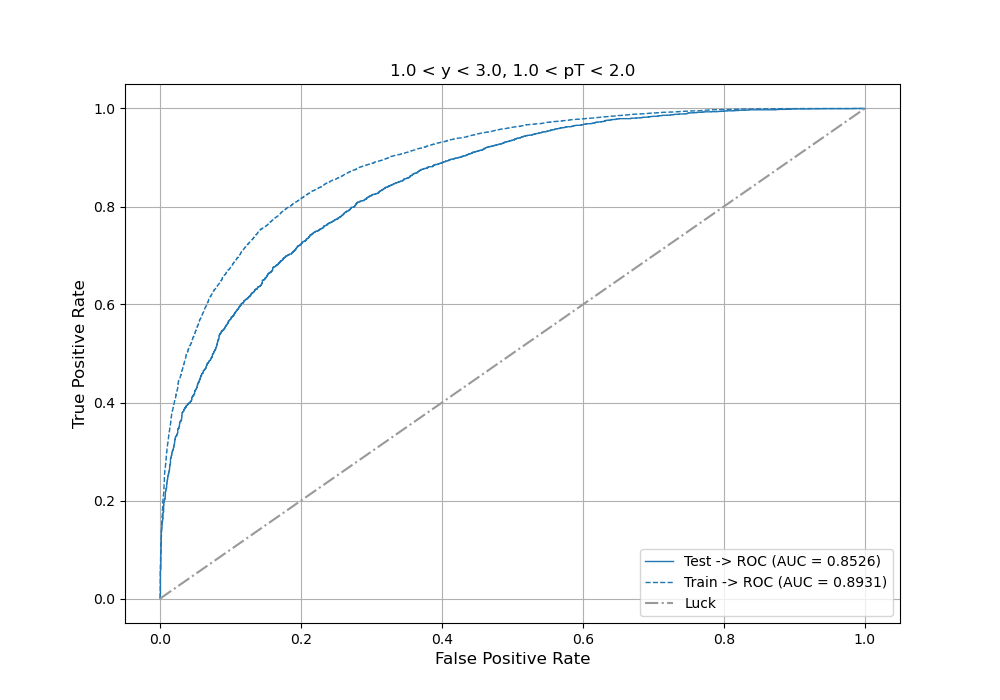
\includegraphics[width=0.5\linewidth]{gallery/results2/fav_roc_train_test.png}
    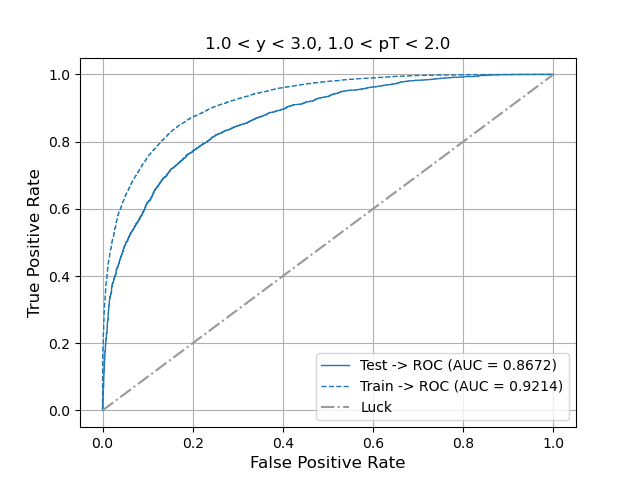
\includegraphics[width=0.46\linewidth]{gallery/results2/fav_roc_train_test_5params.png}
    \caption{ROC curves for training data (dashed line) and testing data (solid line) for BDTs with different hyperparameter optimization condition, in $1<y<3$ and $1<p_T<2~{\rm GeV/c}$. The left plot shows results for case I (Test AUC = 0.8526, Train AUC = 0.8931), and the right plot shows results for case III (Test AUC = 0.8672, Train AUC = 0.9214).}
    \label{f.bdt_hyperparams}
\end{figure}
%
In case III (right plot), we observe greater discrepancies in the ROC curves and AUC values between training and testing data. Even with increased regularization via \texttt{min\_child\_weight} and \texttt{min\_split\_loss}, the high values for the basic hyperparameters are enough to cause overfitting. We do also observe a higher AUC value for the testing data in case III (0.8672) than in case I (0.8526), which suggests that the model which overfits the training data does perform slightly better on testing data. 

It is likely the case that BDT performance does not drop significantly with increased overfitting \cite{BDT}, which may explain Optuna's tendency to find hyperparameter values that overfit. Based on these results, we favor the use of the more restrictive ranges for the basic hyperparameters, as in case I. Alternatively, stronger regularization may also work to prevent overfitting.

%
% \begin{figure}[h!]
%     \centering
%     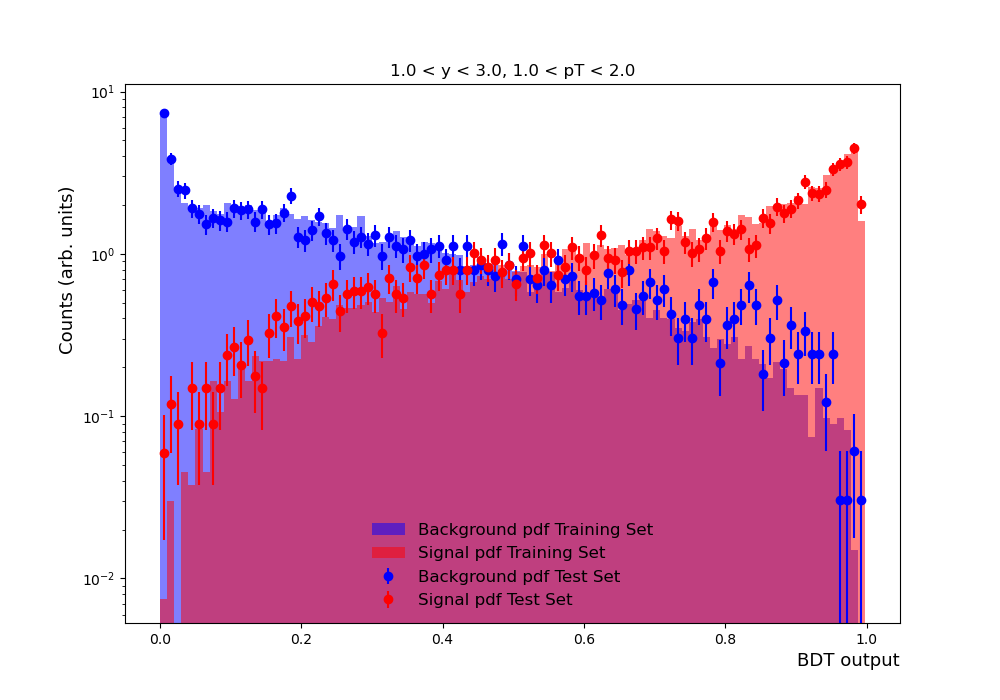
\includegraphics[width=0.5\linewidth]{gallery/results2/fav_train_test.png}
%     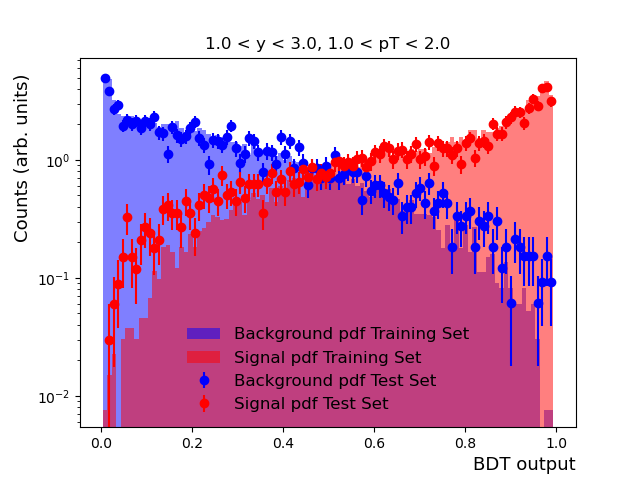
\includegraphics[width=0.46\linewidth]{gallery/results2/fav_train_test_5params.png}
%     \caption{BDT output distributions of training vs. test data for samples without (left) and \textbf{with (right)} machine-background effects. In both plots, training data are plotted as shaded histograms and test data are plotted as solid markers, with background candidates in blue and $D^0$ signal candidates in red.}
%     \label{f.roc_hyperparams}
% \end{figure}
%

%---------------------------------------------------------
\section{Comparison of BDT based method to non-ML analysis}
\label{sec.results_box_cuts}

Finally, we conclude our analysis with a comparison of BDT results to the box cuts on topological features, which we would normally apply for non-machine learning based studies. Focusing on $-1<y<1$ and $2<p_T<3~{\rm GeV/c}$ as an example, we obtain the box cuts from a previous $D^0$ analysis by the STAR Collaboration \cite{STAR}, which we list in Table \ref{tab.box_cuts}. We then train a BDT model using the six features for the same kinematic slice.

\begin{table}[h!]
    \centering
    \begin{tabular}{l|c}
         Feature & Cut \\
         \hline
         Decay Length (mm) & $>0.232$ \\
         ${\rm DCA_{12}}$ (mm) & $<0.063$ \\
         ${\rm DCA_{D0}}$ (mm) & $<0.040$ \\
         ${\rm DCA_{\pi}}$ (mm) & $>0.097$ \\
         ${\rm DCA_{K}}$ (mm) & $>0.094$ \\
         $\cos{\theta}$ & $>0.95$
    \end{tabular}
    \caption{Box cuts on $D^0\rightarrow\pi+K$ topology for $-1<y<1$ and $2<p_T<3~{\rm GeV/c}$, from the STAR Collaboration \cite{STAR}.}
    \label{tab.box_cuts}
\end{table}

%
\begin{figure}[h!]
    \centering
    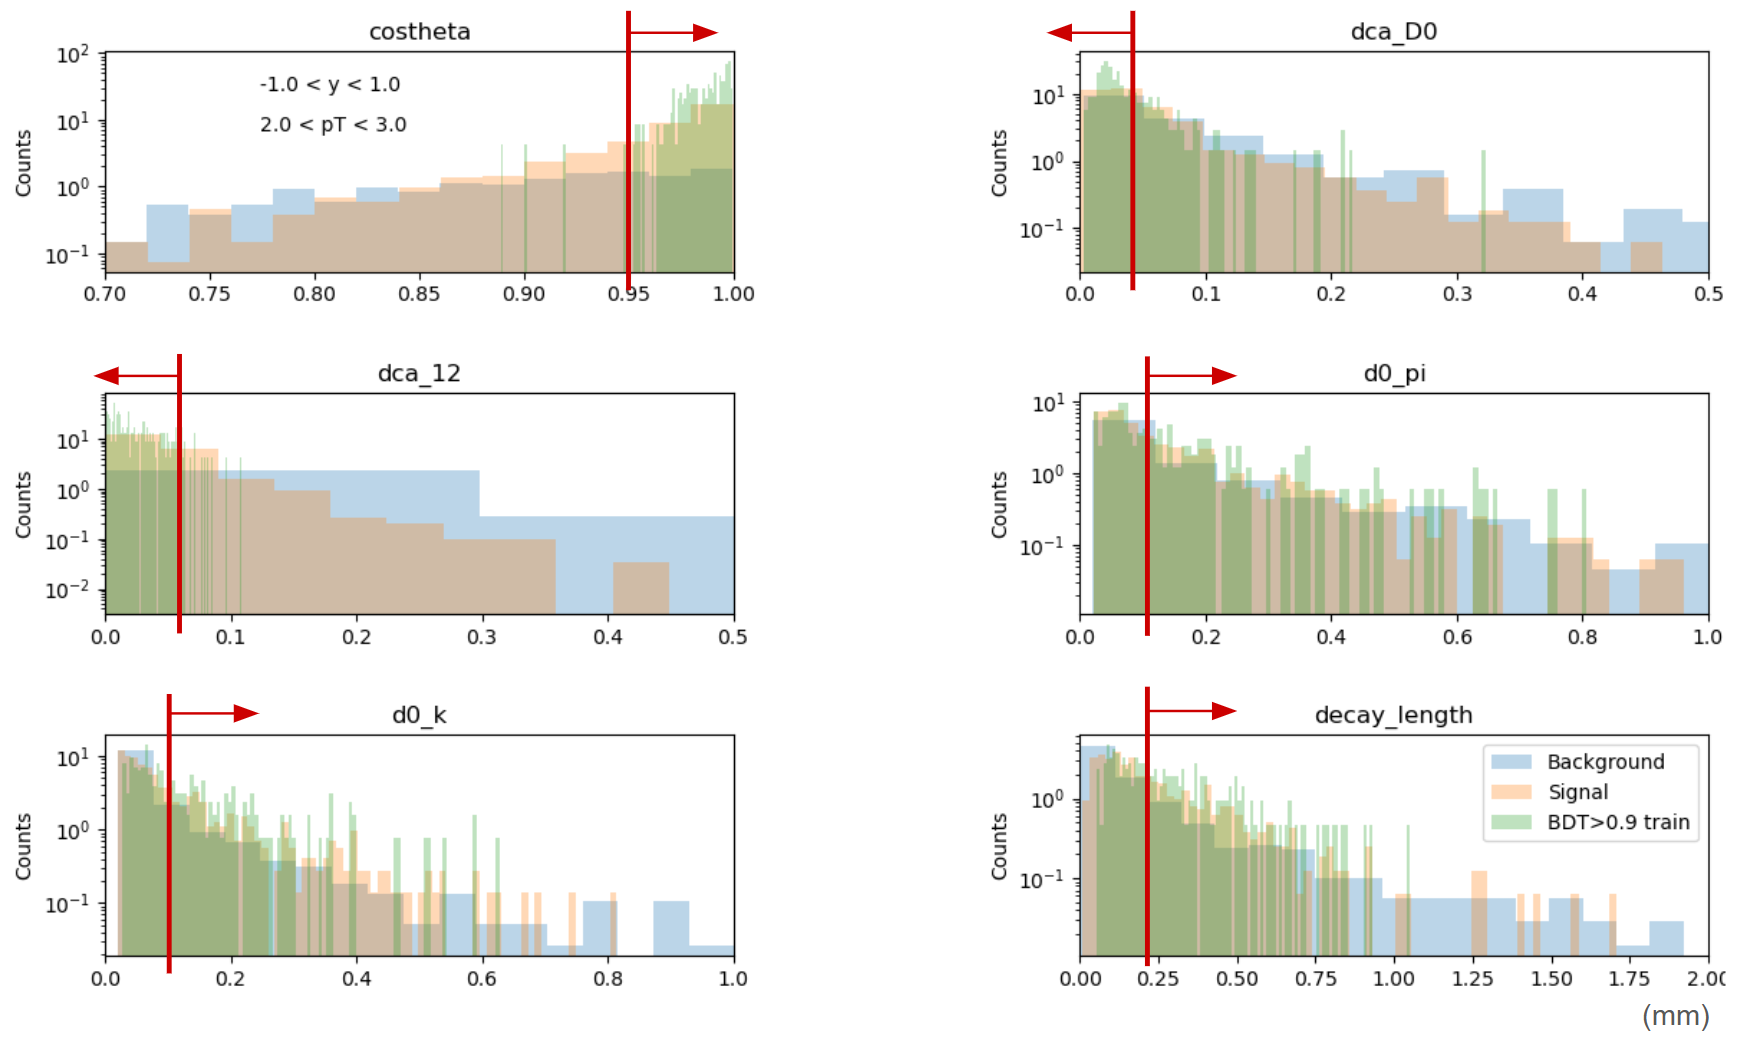
\includegraphics[width=0.9\linewidth]{gallery/results2/top_BDT_vs_box.png}
    \caption{Topological distributions of candidates in the training dataset for $-1<y<1$ and $2<p_T<3~{\rm GeV/c}$, comparing true signal candidates (orange), true background candidates (blue), candidates selected for BDT output $>0.9$ (green), and candidates selected by box cuts (red arrow) from the STAR Collaboration analysis \cite{STAR}.}
    \label{f.bdt_vs_box}
\end{figure}
%
In Fig. \ref{f.bdt_vs_box}, we plot the topological distributions of the true signal candidates (orange) and true background candidates (blue) in the training data, along with the candidates accepted by the BDT for a threshold of 0.9 (green) and those accepted by the box cuts in Table \ref{tab.box_cuts} (red arrows). We choose the BDT threshold value to yield the most similar S/B ratio as that obtained using the box cuts, and we obtain the selected candidates by applying the model onto its training data (without additional resampling). Comparing the BDT selections and box cuts, we observe that both generally favor candidates toward the same side of each distributions. For example, both tend to accept candidates with high values of $\cos{\theta}$, low values of ${\rm DCA_{D0}}$, low values of ${\rm DCA_{12}}$, etc. However, the BDT selections are much more flexible than the hard cutoffs of the box cuts. 

Interestingly, we observe that the BDT selections and box cuts are quite similar for $\cos{\theta}$ and ${\rm DCA_{12}}$, which are the two most important features according to the mean SHAP values. These selections also make sense intuitively, since we expect perfectly reconstructed $D^0$ signals to have $\cos{\theta}=1$ and ${\rm DCA_{12}}=0$. These observations offer some confidence that the BDT is learning the true signal-and-background boundaries, consistent with what we can expect from our physical intuition and from non-ML methods of analysis. 

%
\begin{figure}[h!]
    \centering
    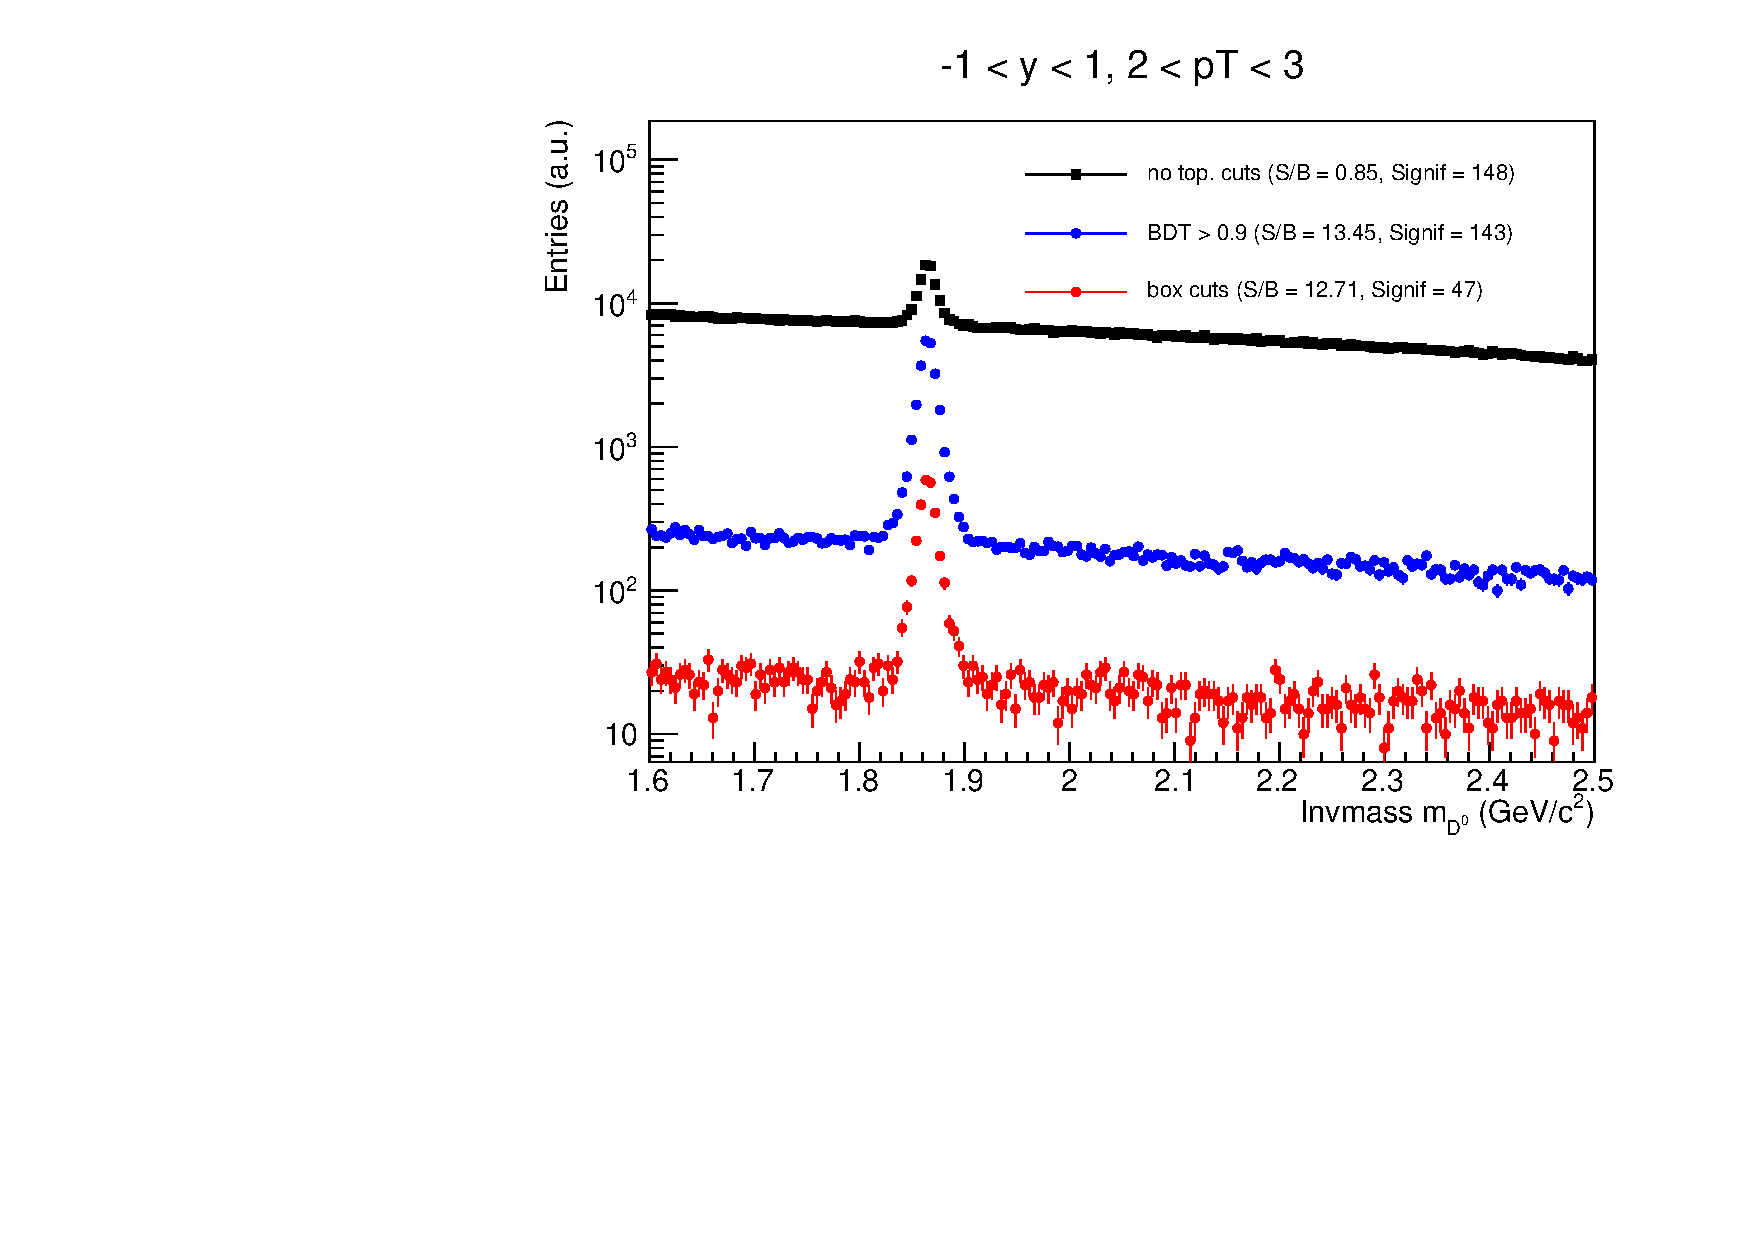
\includegraphics[width=0.65\linewidth]{gallery/results2/inv_mass_ML_vs_box_cuts_y_-1.0_1.0_pt_2.0_3.0_bdt_0.9.pdf}
    \caption{Reconstructed $D^0$ invariant mass distributions before BDT (black), after applying box cuts (red), and after applying BDTs selections (blue), for $2<p_T<3~{\rm GeV/c}$. The BDT threshold is selected to yield the S/B most similar to that of the box cuts.}
    \label{f.inv_mass_box}
\end{figure}
%
Comparing the $D^0$ invariant mass distributions in Fig. \ref{f.inv_mass_box}, we find that for similar S/B values, the BDT selections yield a much greater Significance than the box cuts. The ability of the BDT to preserve higher statistics and thus produce higher Significance illustrates an important advantage of the ML method over traditional box cuts.